\documentclass[12pt,a4paper,oneside]{report}
% Compile with XeLaTeX. UTF-8 sources.
\usepackage{fontspec}
\usepackage{polyglossia}
\setmainlanguage{ukrainian}
\setotherlanguage{english}
\setmainfont{Libertinus Serif}
\setsansfont{Libertinus Sans}
\setmonofont{Libertinus Mono}
\usepackage{amsmath}
\usepackage{unicode-math}
\setmathfont{Libertinus Math}
\usepackage[a4paper,left=25mm,right=20mm,top=23mm,bottom=23mm]{geometry}
\usepackage{graphicx}
\usepackage{tikz}
\graphicspath{{figures/}}
\usepackage{booktabs,array,tabularx}
\usepackage{siunitx}
\sisetup{output-decimal-marker={,}}
\usepackage{caption,subcaption}
\captionsetup{font=small,labelfont=bf}
\usepackage{microtype}
\usepackage{setspace}
\setstretch{1.12}
\setlength{\parindent}{1.25cm}
\setlength{\parskip}{0pt}
\usepackage{titlesec}
\titleformat{\chapter}[hang]{\normalfont\Large\bfseries}{\thechapter.}{0.7em}{}
\titlespacing*{\chapter}{0pt}{0pt}{1.2em}
\newif\ifreportbibliography
% Enable only after verified references and citations are added:
% \reportbibliographytrue
\ifreportbibliography
  \usepackage[backend=biber,style=numeric,sorting=none]{biblatex}
  \addbibresource{references.bib}
\fi
\usepackage[unicode,hidelinks]{hyperref}
% Visible placeholders are never evidence or scientific claims.
\newcommand{\reporttodo}[1]{\par\noindent\textit{Робочий план: #1}\par}

% Shared notation; review against evidence in G2-SR0.
\newcommand{\KI}{K_{\mathrm{I}}}
\newcommand{\KII}{K_{\mathrm{II}}}
\newcommand{\FG}{F_G}
\newcommand{\Eeff}{E'}
\newcommand{\deltacrack}{\Delta a}
\newcommand{\pathH}{\Gamma_{\mathrm{H}}}
\newcommand{\pathM}{\Gamma_{\mathrm{M}}}

\title{Керування рушійною силою та траєкторією поширення тріщини в метакомпозитах}
\author{Інститут механіки ім.~С.~П.~Тимошенка НАН України}
\date{Робоча редакція --- 25 листопада 2026 р.}
\begin{document}
\maketitle
\noindent\textbf{Статус:} G2-SR0, робоча редакція. Розділи 2--7 підготовлено для наукового розгляду; решта розділів --- каркас.
\tableofcontents
\chapter{Вступ. Сучасний стан проблеми та наукові прогалини}
\label{ch:introduction}
\reporttodo{Огляд літератури; формулювання задачі та перевірюваних гіпотез.}

\chapter{Постановка задачі}
\label{ch:problem}
\reporttodo{Геометрія, матеріали, граничні умови та ідеалізація модельного зразка.}

\chapter{Методика чисельного дослідження}
\label{ch:methods}
\reporttodo{Дискретизація, побудова сіток, COD, EDI, критерій МКН та алгоритм розвитку тріщини.}

\chapter{Верифікація чисельної методики}
\label{ch:verification}
\reporttodo{Незалежні оцінки КІН, сіткова чутливість та межі застосовності.}

\chapter{Вплив матеріальної неоднорідності за заданої геометрії тріщини}
\label{ch:fixed-crack}

Перш ніж будувати траєкторії тріщини в метакомпозиті, необхідно встановити, як зміна пружних характеристик кілець впливає на розв'язок при незмінній геометрії тріщини. Це дає змогу відокремити прямий матеріальний ефект від зміни розв'язку, спричиненої поворотом та подовженням тріщини. У цьому розділі розглядаємо найпростіший варіант матеріальної архітектури: модулі всіх трьох кілець змінюються одночасно і в однаковій пропорції. З'ясуємо, чи зберігаються знак і величина впливу кілець при наближенні вершини до області неоднорідності, а також чи можна передбачити цей вплив за зміною інтегральної жорсткості пластини.

\section{Схема розрахункового експерименту}
\label{sec:fixed-design}

Вихідними є три геометрії тріщини, отримані для однорідної перфорованої пластини: початкова пряма тріщина S0 та дві ламані після одного і двох приростів за критерієм МКН (S1 і S2). Довжини тріщин становлять 25,4; 29,4 та 33,4 мм. На кожній з цих геометрій розв'язуємо крайову задачу для трьох розподілів модулів:
\begin{equation}
 \boldsymbol\lambda_{\mathrm H}=(1,1,1),\qquad
 \boldsymbol\lambda_{\mathrm s}=(0{,}5,0{,}5,0{,}5),\qquad
 \boldsymbol\lambda_{\mathrm r}=(2,2,2).
 \label{eq:fixed-architectures}
\end{equation}
Позначення s і r у нижніх індексах стосуються відповідно м'яких і жорстких кілець; аргумент $s$ надалі означає довжину тріщини. Ці конфігурації з трьома активними кільцями не слід ототожнювати з soft1, soft2 та stiff13, які мають інше розташування активних областей.

У межах кожної геометрії використовуємо однакову сітку, крайові умови та силу $P=1$ Н. Змінюємо лише матеріальні характеристики елементів кілець. Однорідний розв'язок, отриманий за допомогою багатофазної реалізації при $\lambda_i=1$, побітово відтворює відповідний однорідний розв'язок. Отже, мітки матеріальних областей самі по собі не створюють чисельного контрасту. Усі три геометрії мають однакову дискретну площу кільця $1012{,}152529$ мм$^2$ та 76 хорд на його зовнішній межі. Однак зовнішня сітка змінюється від стану до стану, а S0 належить до початкового сімейства сіток прямої тріщини.

\begin{figure}[htbp]
 \centering
 % Nominal rings; reference tips from WP34_STATE2_RESULTS.md.
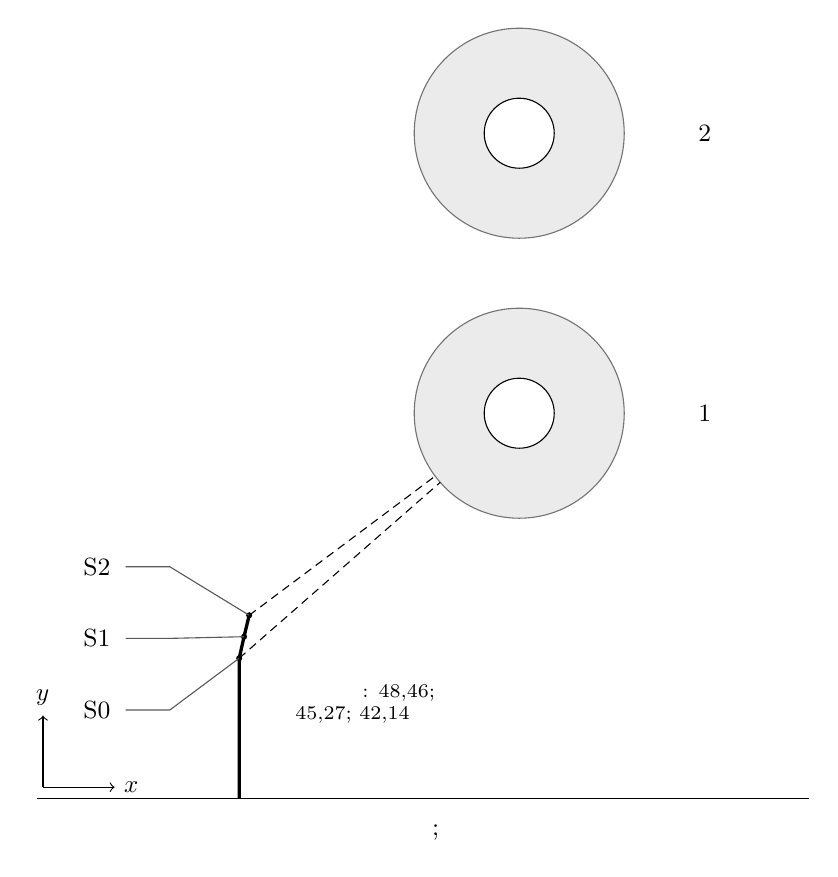
\begin{tikzpicture}[x=.7mm,y=.7mm,font=\small]
 \draw (65,0)--(205,0);
 \foreach \yy in {69.85,120.65}{
   \filldraw[fill=black!8,draw=black!55] (152.4,\yy) circle[radius=19.05];
   \filldraw[fill=white,draw=black] (152.4,\yy) circle[radius=6.35];
 }
 \node[anchor=west] at (174,69.85) {Кільце 1};
 \node[anchor=west] at (174,120.65) {Кільце 2};
 \draw[very thick] (101.6,0)--(101.6,25.4)--(102.4722795671,29.3037326185)--(103.4091509165,33.1924691839);
 \foreach \xx/\yy/\lab/\ly in {101.6/25.4/S0/16,102.4722795671/29.3037326185/S1/29,103.4091509165/33.1924691839/S2/42}{
   \fill (\xx,\yy) circle[radius=1.1pt];
   \draw[black!65] (\xx,\yy)--(89,\ly)--(81,\ly);
   \node[anchor=east] at (80,\ly) {\lab};
 }
 \draw[densely dashed] (101.6,25.4)--(138.06341397,57.30548722);
 \draw[densely dashed] (103.4091509165,33.1924691839)--(137.14721633,58.43706477);
 \node[anchor=west,align=left,font=\scriptsize] at (110,18) {Відстані до найближчого\\вузла кільця: 48,46;\\45,27; 42,14 мм};
 \draw[->] (66,2)--(79,2) node[anchor=west] {$x$};
 \draw[->] (66,2)--(66,15) node[anchor=south] {$y$};
 \node[anchor=north] at (135,-3) {Фрагмент пластини; розміри в мм};
\end{tikzpicture}

 \caption{Три зафіксовані геометрії тріщини в однорідній пластині та їхнє положення відносно нижніх кілець. Номінальні кругові контури й штрихові лінії показано схематично; відстані наведено за фактичними вузлами сітки.}
 \label{fig:fixed-geometry}
\end{figure}

Як видно з рис.~\ref{fig:fixed-geometry}, тріщина ще не наближається до міжфазної межі настільки, щоб вона впливала на допустимість привершинної області. Відстань до найближчого вузла кільця зменшується з 48,46 до 42,14 мм, а запас відносно номінального зовнішнього радіуса інтегрування 2,6 мм залишається більшим за 39 мм. Тому розглянуті зміни КІН є результатом перерозподілу пружних полів у пластині, а не зміни локального матеріалу вершини.

\section{Екранування та підсилення рушійної сили}
\label{sec:fixed-energy}

Відносний ефект визначаємо за~\eqref{eq:problem-fixed-contrast}. Для зручності позначимо $R_{\mathrm{mat}}=1+F_G^{\mathrm{fix}}$. У таблиці~\ref{tab:fixed-energy} наведено основні EDI-значення контрастів та два прийняті показники чисельної невизначеності, визначені в розділі~\ref{ch:verification}. Усі значення $F_G$ наведено у відсотках, а $U_{\mathrm{prim}}$ та $U_{\mathrm{cons}}$ --- у безрозмірних одиницях.

\begin{table}[htbp]
 \centering
 \caption{Прямий матеріальний ефект для трьох зафіксованих геометрій}
 \label{tab:fixed-energy}
 \begin{tabular}{llrrr}
 \toprule
 Стан & Кільця & $F_G$, \% & $U_{\mathrm{prim}}$ & $U_{\mathrm{cons}}$\\
 \midrule
 S0 & М'які & $-0,6093$ & $9,385\cdot10^{-6}$ & 0,0349\\
    & Жорсткі & $-0,9040$ & $6,839\cdot10^{-6}$ & 0,0349\\
 S1 & М'які & $+0,6199$ & $4,699\cdot10^{-6}$ & 0,0352\\
    & Жорсткі & $-1,8130$ & $2,586\cdot10^{-6}$ & 0,0344\\
 S2 & М'які & $+2,1813$ & $1,303\cdot10^{-6}$ & 0,0358\\
    & Жорсткі & $-2,9313$ & $4,968\cdot10^{-8}$ & 0,0340\\
 \bottomrule
 \end{tabular}
\end{table}

\begin{figure}[htbp]
 \centering
 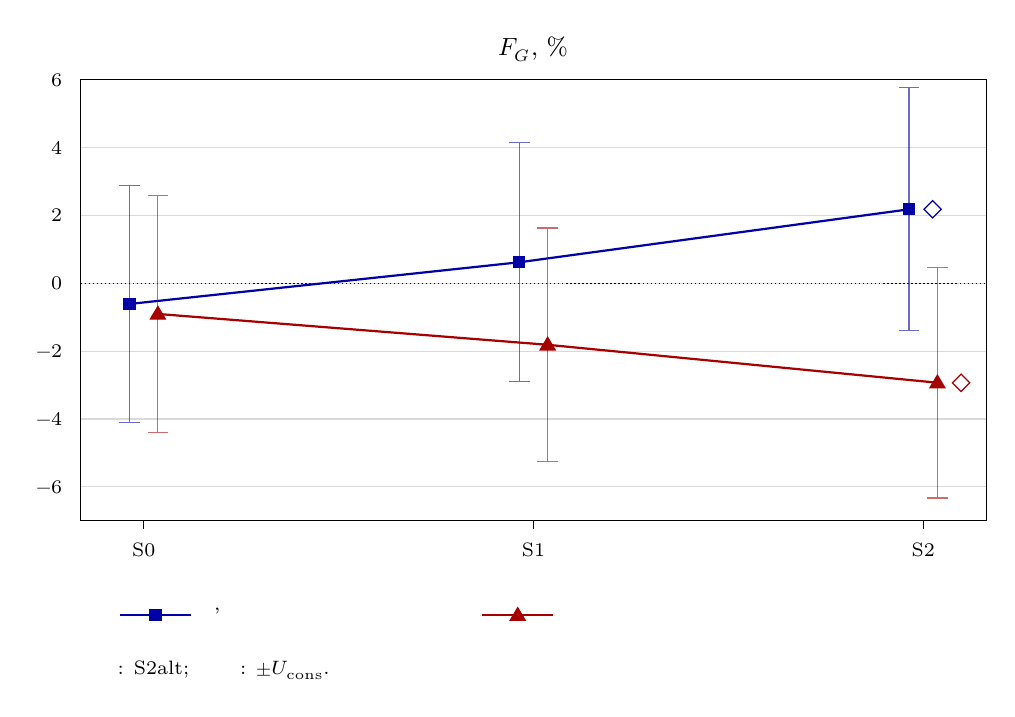
\begin{tikzpicture}[x=1mm,y=1mm,font=\small,line width=.45pt]
\draw[black!15] (0,4.3077)--(115,4.3077);\node[anchor=east,font=\scriptsize] at (-1,4.3077) {$-6$};
\draw[black!15] (0,12.9231)--(115,12.9231);\node[anchor=east,font=\scriptsize] at (-1,12.9231) {$-4$};
\draw[black!15] (0,21.5385)--(115,21.5385);\node[anchor=east,font=\scriptsize] at (-1,21.5385) {$-2$};
\draw[black!15] (0,30.1538)--(115,30.1538);\node[anchor=east,font=\scriptsize] at (-1,30.1538) {$0$};
\draw[black!15] (0,38.7692)--(115,38.7692);\node[anchor=east,font=\scriptsize] at (-1,38.7692) {$2$};
\draw[black!15] (0,47.3846)--(115,47.3846);\node[anchor=east,font=\scriptsize] at (-1,47.3846) {$4$};
\draw[black!15] (0,56)--(115,56);\node[anchor=east,font=\scriptsize] at (-1,56) {$6$};
\draw[densely dotted] (0,30.1538)--(115,30.1538);
\draw (0,0) rectangle (115,56);\node[anchor=south] at (57.5,57) {$F_G$, \%};
\draw (8,0)--(8,-1);\node[anchor=north,font=\scriptsize] at (8,-1.5) {S0};
\draw (57.5,0)--(57.5,-1);\node[anchor=north,font=\scriptsize] at (57.5,-1.5) {S1};
\draw (107,0)--(107,-1);\node[anchor=north,font=\scriptsize] at (107,-1.5) {S2};
\draw[blue!65!black,opacity=.58] (6.2,12.4953)--(6.2,42.563) (4.9,12.4953)--(7.5,12.4953) (4.9,42.563)--(7.5,42.563);
\draw[blue!65!black,opacity=.58] (55.7,17.661)--(55.7,47.9872) (54.4,17.661)--(57,17.661) (54.4,47.9872)--(57,47.9872);
\draw[blue!65!black,opacity=.58] (105.2,24.1288)--(105.2,54.9718) (103.9,24.1288)--(106.5,24.1288) (103.9,54.9718)--(106.5,54.9718);
\draw[blue!65!black,line width=.8pt] (6.2,27.5291)--(55.7,32.8241)--(105.2,39.5503);
\draw[blue!65!black,fill=blue!65!black] (5.5,26.8291) rectangle (6.9,28.2291);
\draw[blue!65!black,fill=blue!65!black] (55,32.1241) rectangle (56.4,33.5241);
\draw[blue!65!black,fill=blue!65!black] (104.5,38.8503) rectangle (105.9,40.2503);
\draw[blue!65!black,fill=white] (108.2,40.6566)--(109.3,39.5566)--(108.2,38.4566)--(107.1,39.5566)--cycle;
\draw[red!65!black,opacity=.58] (9.8,11.2258)--(9.8,41.2935) (8.5,11.2258)--(11.1,11.2258) (8.5,41.2935)--(11.1,41.2935);
\draw[red!65!black,opacity=.58] (59.3,7.5256)--(59.3,37.1625) (58,7.5256)--(60.6,7.5256) (58,37.1625)--(60.6,37.1625);
\draw[red!65!black,opacity=.58] (108.8,2.8807)--(108.8,32.173) (107.5,2.8807)--(110.1,2.8807) (107.5,32.173)--(110.1,32.173);
\draw[red!65!black,line width=.8pt] (9.8,26.2597)--(59.3,22.3441)--(108.8,17.5268);
\draw[red!65!black,fill=red!65!black] (9.8,27.2097)--(8.85,25.6097)--(10.75,25.6097)--cycle;
\draw[red!65!black,fill=red!65!black] (59.3,23.2941)--(58.35,21.6941)--(60.25,21.6941)--cycle;
\draw[red!65!black,fill=red!65!black] (108.8,18.4768)--(107.85,16.8768)--(109.75,16.8768)--cycle;
\draw[red!65!black,fill=white] (111.8,18.6183)--(112.9,17.5183)--(111.8,16.4183)--(110.7,17.5183)--cycle;
\draw[blue!65!black,line width=.8pt] (5,-12)--(14,-12);
\draw[blue!65!black,fill=blue!65!black] (8.8,-12.7) rectangle (10.2,-11.3);
\node[anchor=west,font=\scriptsize] at (15,-12) {М'які кільця};
\draw[red!65!black,line width=.8pt] (51,-12)--(60,-12);
\draw[red!65!black,fill=red!65!black] (55.5,-11.05)--(54.55,-12.65)--(56.45,-12.65)--cycle;
\node[anchor=west,font=\scriptsize] at (61,-12) {Жорсткі кільця};
\node[anchor=west,font=\scriptsize] at (0,-19) {Ромби: S2alt; відрізки: $\pm U_{\mathrm{cons}}$.};
\end{tikzpicture}

 \caption{Енергетичний контраст за незмінної геометрії тріщини. Відрізки показують консервативний показник $\pm U_{\mathrm{cons}}$, а не довірчі інтервали; первинний розкид наведено в табл.~\ref{tab:fixed-energy}. Лінії лише з'єднують дискретні результати; ромби відповідають альтернативній сітці S2alt.}
 \label{fig:fixed-contrast}
\end{figure}

При збільшенні модуля Юнга кілець у два рази отримано від'ємні контрасти на всіх трьох геометріях, причому їхні модулі зростають. При зменшенні модуля вдвічі отримано іншу поведінку: від'ємне значення на S0 змінюється додатним на S1 і зростає на S2. Таким чином, для однієї і тієї самої неоднорідності знак обчисленої зміни рушійної сили залежить від геометрії тріщини. За трьома дискретними точками не можна визначити точну довжину, за якої відбувається зміна знака, або довести монотонність між ними.

Усі шість контрастів розрізняються за первинним критерієм $|F_G|>2U_{\mathrm{prim}}$, причому знаки за COD та EDI збігаються. Проте жоден не розрізняється за консервативним критерієм $|F_G|>U_{\mathrm{cons}}$. Це стосується саме раннього дослідження трьох однаково активованих кілець. На S2 додатково перевірено обидва контрасти на незалежно перебудованій зовнішній сітці з 112 хордами: для м'яких кілець $+2{,}1813\to+2{,}1828$\,\%, для жорстких $-2{,}9313\to-2{,}9333$\,\%. Спостережена зміна становить близько 0,07\,\% від величини відповідного ефекту. Цей результат підтримує стійкість контрастів на S2, але не є прямою перевіркою сіткової чутливості для S0 і S1 та не скасовує консервативного висновку.

\section{Внески двох мод руйнування}
\label{sec:fixed-modes}

Щоб зрозуміти причину зміни енергетичного контрасту, розглянемо окремі внески КІН. Для будь-якої з фіксованих геометрій позначимо однорідні КІН через $A=K_{\mathrm I,H}$ та $B_K=K_{\mathrm{II},H}$, а зміни в неоднорідному матеріалі --- через $\Delta\KI$ та $\Delta\KII$. Оскільки матеріал вершини незмінний, з~\eqref{eq:problem-G} випливає точна тотожність
\begin{equation}
 \begin{aligned}
 F_G={}&F_{\mathrm I}+F_{\mathrm{II}},\\
 F_{\mathrm I}={}&\frac{2A\Delta\KI+(\Delta\KI)^2}{A^2+B_K^2},\\
 F_{\mathrm{II}}={}&\frac{2B_K\Delta\KII+(\Delta\KII)^2}{A^2+B_K^2}.
 \end{aligned}
 \label{eq:fixed-mode-decomp}
\end{equation}
Тут $F_{\mathrm I}$ та $F_{\mathrm{II}}$ є змінами відповідних модових складових енергії, нормованими на повне опорне $G$. Це алгебраїчний розклад, а не розділення просторових механізмів перерозподілу напружень.

\begin{figure}[htbp]
 \centering
 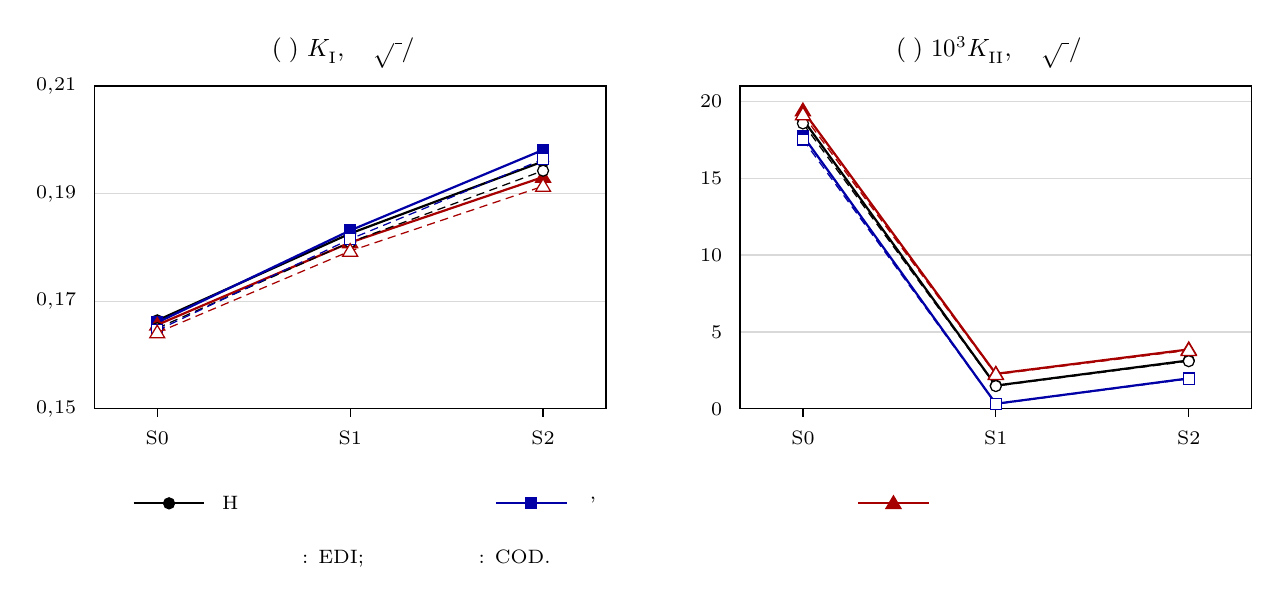
\begin{tikzpicture}[x=1mm,y=1mm,font=\small,line width=.45pt]
\draw[black!15] (0,0)--(65,0);\node[anchor=east,font=\scriptsize] at (-1,0) {$0{,}15$};
\draw[black!15] (0,13.6667)--(65,13.6667);\node[anchor=east,font=\scriptsize] at (-1,13.6667) {$0{,}17$};
\draw[black!15] (0,27.3333)--(65,27.3333);\node[anchor=east,font=\scriptsize] at (-1,27.3333) {$0{,}19$};
\draw[black!15] (0,41)--(65,41);\node[anchor=east,font=\scriptsize] at (-1,41) {$0{,}21$};
\draw (0,0) rectangle (65,41);\node[anchor=south] at (32.5,42) {(а) $K_{\mathrm I}$, МПа$\sqrt{\text{м}}$/кН};
\draw (8,0)--(8,-1);\node[anchor=north,font=\scriptsize] at (8,-1.5) {S0};
\draw (32.5,0)--(32.5,-1);\node[anchor=north,font=\scriptsize] at (32.5,-1.5) {S1};
\draw (57,0)--(57,-1);\node[anchor=north,font=\scriptsize] at (57,-1.5) {S2};
\draw[black,line width=.8pt] (8,11.2312)--(32.5,22.2663)--(57,31.4213);
\draw[black,fill=black] (8,11.2312) circle[radius=.7mm];
\draw[black,fill=black] (32.5,22.2663) circle[radius=.7mm];
\draw[black,fill=black] (57,31.4213) circle[radius=.7mm];
\draw[blue!65!black,line width=.8pt] (8,10.9597)--(32.5,22.6565)--(57,32.8847);
\draw[blue!65!black,fill=blue!65!black] (7.3,10.2597) rectangle (8.7,11.6597);
\draw[blue!65!black,fill=blue!65!black] (31.8,21.9565) rectangle (33.2,23.3565);
\draw[blue!65!black,fill=blue!65!black] (56.3,32.1847) rectangle (57.7,33.5847);
\draw[red!65!black,line width=.8pt] (8,10.6639)--(32.5,21.1246)--(57,29.4345);
\draw[red!65!black,fill=red!65!black] (8,11.6139)--(7.05,10.0139)--(8.95,10.0139)--cycle;
\draw[red!65!black,fill=red!65!black] (32.5,22.0746)--(31.55,20.4746)--(33.45,20.4746)--cycle;
\draw[red!65!black,fill=red!65!black] (57,30.3845)--(56.05,28.7845)--(57.95,28.7845)--cycle;
\draw[black,densely dashed] (8,10.234)--(32.5,21.1692)--(57,30.2443);
\draw[black,fill=white] (8,10.234) circle[radius=.7mm];
\draw[black,fill=white] (32.5,21.1692) circle[radius=.7mm];
\draw[black,fill=white] (57,30.2443) circle[radius=.7mm];
\draw[blue!65!black,densely dashed] (8,9.9648)--(32.5,21.5556)--(57,31.6947);
\draw[blue!65!black,fill=white] (7.3,9.2648) rectangle (8.7,10.6648);
\draw[blue!65!black,fill=white] (31.8,20.8556) rectangle (33.2,22.2556);
\draw[blue!65!black,fill=white] (56.3,30.9947) rectangle (57.7,32.3947);
\draw[red!65!black,densely dashed] (8,9.6718)--(32.5,20.0377)--(57,28.275);
\draw[red!65!black,fill=white] (8,10.6218)--(7.05,9.0218)--(8.95,9.0218)--cycle;
\draw[red!65!black,fill=white] (32.5,20.9877)--(31.55,19.3877)--(33.45,19.3877)--cycle;
\draw[red!65!black,fill=white] (57,29.225)--(56.05,27.625)--(57.95,27.625)--cycle;
\draw[black!15] (82,0)--(147,0);\node[anchor=east,font=\scriptsize] at (81,0) {$0$};
\draw[black!15] (82,9.7619)--(147,9.7619);\node[anchor=east,font=\scriptsize] at (81,9.7619) {$5$};
\draw[black!15] (82,19.5238)--(147,19.5238);\node[anchor=east,font=\scriptsize] at (81,19.5238) {$10$};
\draw[black!15] (82,29.2857)--(147,29.2857);\node[anchor=east,font=\scriptsize] at (81,29.2857) {$15$};
\draw[black!15] (82,39.0476)--(147,39.0476);\node[anchor=east,font=\scriptsize] at (81,39.0476) {$20$};
\draw (82,0) rectangle (147,41);\node[anchor=south] at (114.5,42) {(б) $10^3 K_{\mathrm{II}}$, МПа$\sqrt{\text{м}}$/кН};
\draw (90,0)--(90,-1);\node[anchor=north,font=\scriptsize] at (90,-1.5) {S0};
\draw (114.5,0)--(114.5,-1);\node[anchor=north,font=\scriptsize] at (114.5,-1.5) {S1};
\draw (139,0)--(139,-1);\node[anchor=north,font=\scriptsize] at (139,-1.5) {S2};
\draw[black,line width=.8pt] (90,36.7576)--(114.5,2.9552)--(139,6.1499);
\draw[black,fill=black] (90,36.7576) circle[radius=.7mm];
\draw[black,fill=black] (114.5,2.9552) circle[radius=.7mm];
\draw[black,fill=black] (139,6.1499) circle[radius=.7mm];
\draw[blue!65!black,line width=.8pt] (90,34.6852)--(114.5,0.6467)--(139,3.8706);
\draw[blue!65!black,fill=blue!65!black] (89.3,33.9852) rectangle (90.7,35.3852);
\draw[blue!65!black,fill=blue!65!black] (113.8,-0.0533) rectangle (115.2,1.3467);
\draw[blue!65!black,fill=blue!65!black] (138.3,3.1706) rectangle (139.7,4.5706);
\draw[red!65!black,line width=.8pt] (90,37.883)--(114.5,4.4478)--(139,7.5477);
\draw[red!65!black,fill=red!65!black] (90,38.833)--(89.05,37.233)--(90.95,37.233)--cycle;
\draw[red!65!black,fill=red!65!black] (114.5,5.3978)--(113.55,3.7978)--(115.45,3.7978)--cycle;
\draw[red!65!black,fill=red!65!black] (139,8.4977)--(138.05,6.8977)--(139.95,6.8977)--cycle;
\draw[black,densely dashed] (90,36.2526)--(114.5,2.8954)--(139,6.0556);
\draw[black,fill=white] (90,36.2526) circle[radius=.7mm];
\draw[black,fill=white] (114.5,2.8954) circle[radius=.7mm];
\draw[black,fill=white] (139,6.0556) circle[radius=.7mm];
\draw[blue!65!black,densely dashed] (90,34.207)--(114.5,0.6162)--(139,3.8053);
\draw[blue!65!black,fill=white] (89.3,33.507) rectangle (90.7,34.907);
\draw[blue!65!black,fill=white] (113.8,-0.0838) rectangle (115.2,1.3162);
\draw[blue!65!black,fill=white] (138.3,3.1053) rectangle (139.7,4.5053);
\draw[red!65!black,densely dashed] (90,37.3637)--(114.5,4.3693)--(139,7.436);
\draw[red!65!black,fill=white] (90,38.3137)--(89.05,36.7137)--(90.95,36.7137)--cycle;
\draw[red!65!black,fill=white] (114.5,5.3193)--(113.55,3.7193)--(115.45,3.7193)--cycle;
\draw[red!65!black,fill=white] (139,8.386)--(138.05,6.786)--(139.95,6.786)--cycle;
\draw[black,line width=.8pt] (5,-12)--(14,-12);
\draw[black,fill=black] (9.5,-12) circle[radius=.7mm];
\node[anchor=west,font=\scriptsize] at (15,-12) {H};
\draw[blue!65!black,line width=.8pt] (51,-12)--(60,-12);
\draw[blue!65!black,fill=blue!65!black] (54.8,-12.7) rectangle (56.2,-11.3);
\node[anchor=west,font=\scriptsize] at (61,-12) {М'які кільця};
\draw[red!65!black,line width=.8pt] (97,-12)--(106,-12);
\draw[red!65!black,fill=red!65!black] (101.5,-11.05)--(100.55,-12.65)--(102.45,-12.65)--cycle;
\node[anchor=west,font=\scriptsize] at (107,-12) {Жорсткі кільця};
\node[anchor=west,font=\scriptsize] at (0,-19) {Суцільні лінії та заповнені маркери: EDI; штрихові та порожні: COD.};
\end{tikzpicture}

 \caption{Знакові КІН двох мод для трьох геометрій. EDI та COD показано окремо. Значення нормовано на силу 1 кН; на панелі (б) числові значення помножено на $10^3$.}
 \label{fig:fixed-K}
\end{figure}

\begin{table}[htbp]
 \centering
 \caption{Внески мод I та II до зміни рушійної сили (у відсотках від опорного $G$)}
 \label{tab:fixed-modes}
 \begin{tabular}{llrrr}
 \toprule
 Стан & Кільця & $F_{\mathrm I}$ & $F_{\mathrm{II}}$ & $F_G$\\
 \midrule
S0 & М'які & $-0,4709$ & $-0,1385$ & $-0,6093$ \\
S0 & Жорсткі & $-0,9825$ & $0,0785$ & $-0,9040$ \\
S1 & М'які & $0,6264$ & $-0,0065$ & $0,6199$ \\
S1 & Жорсткі & $-1,8217$ & $0,0087$ & $-1,8130$ \\
S2 & М'які & $2,1969$ & $-0,0156$ & $2,1813$ \\
S2 & Жорсткі & $-2,9443$ & $0,0131$ & $-2,9313$ \\
 \bottomrule
 \end{tabular}
\end{table}

Для м'яких кілець на S0 обидві складові від'ємні; зменшення КІН моди II забезпечує близько 23\,\% загального від'ємного контрасту. На S1 і S2 внесок моди I змінює знак, тоді як внесок моди II залишається від'ємним. Отже, обчислений перехід від екранування до підсилення визначається саме зміною КІН моди I, а не зміною знака $\KII$. Для жорстких кілець, навпаки, внесок моди I від'ємний, а моди II додатний на всіх трьох геометріях. Після першого повороту тріщини енергетична зміна майже повністю визначається модою I, хоча модові коефіцієнти II залишаються важливими для визначення напрямку.

Величина $\KII$ на S1 в однорідній пластині становить лише $0{,}001514$ МПа$\sqrt{\text{м}}$ на 1 кН порівняно з $0{,}018827$ на S0. Тому відносна зміна $\KII$ при заміні матеріалу може бути великою навіть за близької абсолютної зміни. Для фізичного тлумачення напрямних ефектів доцільніше розглядати знакові абсолютні зміни та відношення $\KII/\KI$, а не лише відносну зміну другого КІН.

\section{Вплив кілець на локальний напрямок приросту}
\label{sec:fixed-steering}

Позначимо $p=\KII/\KI$ та $\psi=\arctan p$. На кожній геометрії обчислюємо кут МКН за~\eqref{eq:method-mts} в одному й тому самому локальному базисі для всіх трьох матеріалів. Різниця кутів
\begin{equation}
 \Delta\theta=\theta_X-\theta_{\mathrm H}
 \label{eq:fixed-dtheta}
\end{equation}
є прогнозом зміни напрямку наступного приросту, а не різницею вже сформованих траєкторій.

\begin{figure}[htbp]
 \centering
 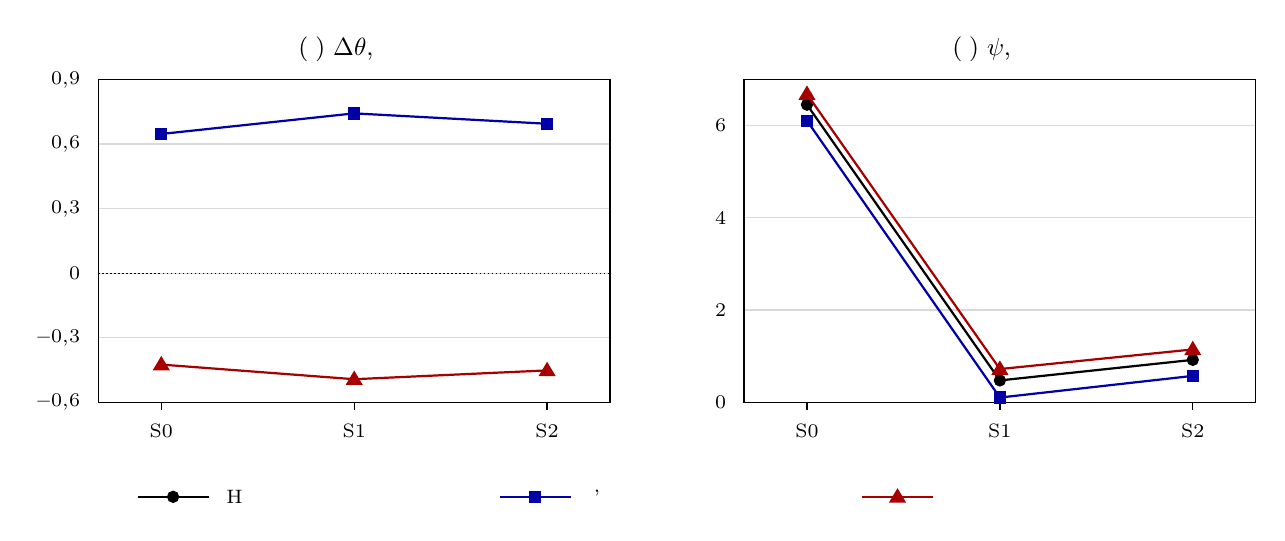
\begin{tikzpicture}[x=1mm,y=1mm,font=\small,line width=.45pt]
\draw[black!15] (0,0)--(65,0);\node[anchor=east,font=\scriptsize] at (-1,0) {$-0{,}6$};
\draw[black!15] (0,8.2)--(65,8.2);\node[anchor=east,font=\scriptsize] at (-1,8.2) {$-0{,}3$};
\draw[black!15] (0,16.4)--(65,16.4);\node[anchor=east,font=\scriptsize] at (-1,16.4) {$0$};
\draw[black!15] (0,24.6)--(65,24.6);\node[anchor=east,font=\scriptsize] at (-1,24.6) {$0{,}3$};
\draw[black!15] (0,32.8)--(65,32.8);\node[anchor=east,font=\scriptsize] at (-1,32.8) {$0{,}6$};
\draw[black!15] (0,41)--(65,41);\node[anchor=east,font=\scriptsize] at (-1,41) {$0{,}9$};
\draw[densely dotted] (0,16.4)--(65,16.4);
\draw (0,0) rectangle (65,41);\node[anchor=south] at (32.5,42) {(а) $\Delta\theta$, град};
\draw (8,0)--(8,-1);\node[anchor=north,font=\scriptsize] at (8,-1.5) {S0};
\draw (32.5,0)--(32.5,-1);\node[anchor=north,font=\scriptsize] at (32.5,-1.5) {S1};
\draw (57,0)--(57,-1);\node[anchor=north,font=\scriptsize] at (57,-1.5) {S2};
\draw[blue!65!black,line width=.8pt] (8,34.0819)--(32.5,36.6975)--(57,35.3779);
\draw[blue!65!black,fill=blue!65!black] (7.3,33.3819) rectangle (8.7,34.7819);
\draw[blue!65!black,fill=blue!65!black] (31.8,35.9975) rectangle (33.2,37.3975);
\draw[blue!65!black,fill=blue!65!black] (56.3,34.6779) rectangle (57.7,36.0779);
\draw[red!65!black,line width=.8pt] (8,4.7956)--(32.5,2.9354)--(57,4.056);
\draw[red!65!black,fill=red!65!black] (8,5.7456)--(7.05,4.1456)--(8.95,4.1456)--cycle;
\draw[red!65!black,fill=red!65!black] (32.5,3.8854)--(31.55,2.2854)--(33.45,2.2854)--cycle;
\draw[red!65!black,fill=red!65!black] (57,5.006)--(56.05,3.406)--(57.95,3.406)--cycle;
\draw[black!15] (82,0)--(147,0);\node[anchor=east,font=\scriptsize] at (81,0) {$0$};
\draw[black!15] (82,11.7143)--(147,11.7143);\node[anchor=east,font=\scriptsize] at (81,11.7143) {$2$};
\draw[black!15] (82,23.4286)--(147,23.4286);\node[anchor=east,font=\scriptsize] at (81,23.4286) {$4$};
\draw[black!15] (82,35.1429)--(147,35.1429);\node[anchor=east,font=\scriptsize] at (81,35.1429) {$6$};
\draw (82,0) rectangle (147,41);\node[anchor=south] at (114.5,42) {(б) $\psi$, град};
\draw (90,0)--(90,-1);\node[anchor=north,font=\scriptsize] at (90,-1.5) {S0};
\draw (114.5,0)--(114.5,-1);\node[anchor=north,font=\scriptsize] at (114.5,-1.5) {S1};
\draw (139,0)--(139,-1);\node[anchor=north,font=\scriptsize] at (139,-1.5) {S2};
\draw[black,line width=.8pt] (90,37.8009)--(114.5,2.782)--(139,5.3934);
\draw[black,fill=black] (90,37.8009) circle[radius=.7mm];
\draw[black,fill=black] (114.5,2.782) circle[radius=.7mm];
\draw[black,fill=black] (139,5.3934) circle[radius=.7mm];
\draw[blue!65!black,line width=.8pt] (90,35.7709)--(114.5,0.6069)--(139,3.3579);
\draw[blue!65!black,fill=blue!65!black] (89.3,35.0709) rectangle (90.7,36.4709);
\draw[blue!65!black,fill=blue!65!black] (113.8,-0.0931) rectangle (115.2,1.3069);
\draw[blue!65!black,fill=blue!65!black] (138.3,2.6579) rectangle (139.7,4.0579);
\draw[red!65!black,line width=.8pt] (90,39.1415)--(114.5,4.2256)--(139,6.7185);
\draw[red!65!black,fill=red!65!black] (90,40.0915)--(89.05,38.4915)--(90.95,38.4915)--cycle;
\draw[red!65!black,fill=red!65!black] (114.5,5.1756)--(113.55,3.5756)--(115.45,3.5756)--cycle;
\draw[red!65!black,fill=red!65!black] (139,7.6685)--(138.05,6.0685)--(139.95,6.0685)--cycle;
\draw[black,line width=.8pt] (5,-12)--(14,-12);
\draw[black,fill=black] (9.5,-12) circle[radius=.7mm];
\node[anchor=west,font=\scriptsize] at (15,-12) {H};
\draw[blue!65!black,line width=.8pt] (51,-12)--(60,-12);
\draw[blue!65!black,fill=blue!65!black] (54.8,-12.7) rectangle (56.2,-11.3);
\node[anchor=west,font=\scriptsize] at (61,-12) {М'які кільця};
\draw[red!65!black,line width=.8pt] (97,-12)--(106,-12);
\draw[red!65!black,fill=red!65!black] (101.5,-11.05)--(100.55,-12.65)--(102.45,-12.65)--cycle;
\node[anchor=west,font=\scriptsize] at (107,-12) {Жорсткі кільця};
\end{tikzpicture}

 \caption{Різниця прогнозованих кутів МКН відносно однорідної пластини (а) та змішаність мод $\psi$ (б) для фіксованих геометрій.}
 \label{fig:fixed-direction}
\end{figure}

На всіх трьох геометріях м'які кільця зменшують модуль від'ємного кута МКН, а жорсткі його збільшують. Для м'яких кілець $\Delta\theta=+0{,}647^\circ$, $+0{,}743^\circ$ та $+0{,}694^\circ$; для жорстких відповідно $-0{,}425^\circ$, $-0{,}493^\circ$ та $-0{,}452^\circ$. Усі шість різниць розрізняються за прийнятим первинним кутовим критерієм, для якого розкид не перевищує $0{,}003^\circ$. На S2 зміна $\Delta\theta$ при заміні зовнішньої сітки не перевищує $2\cdot10^{-4}$ градуса. Це спостереження стосується прогнозу на заданій тріщині.

Математична причина відмінності енергетичного й напрямного ефектів випливає з різної залежності $G$ і $\theta$ від двох КІН. Диференціюючи енергетичне співвідношення при незмінному модулі матриці, отримуємо
\begin{equation}
 \frac{\mathrm dG}{G}=
 \frac{2(\KI\,\mathrm d\KI+\KII\,\mathrm d\KII)}
 {\KI^2+\KII^2}.
 \label{eq:fixed-G-differential}
\end{equation}
Умова стаціонарності МКН~\eqref{eq:method-mts-stationarity} після ділення на $\KI>0$ дає
\begin{equation}
 \frac{\mathrm d\theta}{\mathrm dp}
 =-\frac{3\cos\theta-1}
 {\cos\theta-3p\sin\theta},\qquad
 \mathrm dp=\frac{\mathrm d\KII-p\,\mathrm d\KI}{\KI}.
 \label{eq:fixed-theta-derivative}
\end{equation}
Ці вирази справедливі на регулярній гілці максимуму, де знаменник ненульовий; кут вимірюється в радіанах. Для $|p|\ll1$
\begin{equation}
 \mathrm d\theta\simeq
 -\frac{2}{\KI}(\mathrm d\KII-p\,\mathrm d\KI),\qquad
 \frac{\mathrm dG}{G}\simeq
 \frac{2}{\KI}(\mathrm d\KI+p\,\mathrm d\KII).
 \label{eq:fixed-small-mixity}
\end{equation}
Звідси видно, що за малої змішаності енергетична характеристика переважно чутлива до зміни $\KI$, а напрямна --- до зміни $\KII$. Це локальна математична властивість двох функціоналів, а не твердження про незалежне керування ними через модулі кілець.

Для м'яких кілець абсолютна зміна $\KII$ від S0 до S2 становить $-1{,}0615$, $-1{,}1824$ та $-1{,}1675$ в одиницях $10^{-3}$ МПа$\sqrt{\text{м}}$/кН. Для жорстких --- $+0{,}5764$, $+0{,}7645$ та $+0{,}7159$. Ці зміни зберігають знак, тоді як зміна $\KI$ для м'яких кілець змінює знак. Отже, спостережувана зміна знака енергетичного ефекту при незмінному знаку напрямного ефекту узгоджується з математичною структурою~\eqref{eq:fixed-G-differential} та~\eqref{eq:fixed-theta-derivative}. Причину самого перерозподілу КІН необхідно шукати в полі напружень неоднорідної пластини.

\section{Податливість пластини та енергетична рушійна сила}
\label{sec:fixed-compliance}

Введемо податливість $C=-u_y(\boldsymbol x_P)/P$ за додатної величини спрямованої вниз сили. За незмінної геометрії й лінійно-пружної поведінки повна енергія деформації дорівнює $\mathcal U=P^2C/2$. Якщо $s$ --- довжина тріщини, а похідну взято за її віртуального прямолінійного приросту в локальному напрямку, то при керуванні силою
\begin{equation}
 G=-\frac{1}{t}\frac{\partial\Pi}{\partial s}
 =\frac{P^2}{2t}\frac{\partial C}{\partial s}.
 \label{eq:fixed-compliance-G}
\end{equation}
Тут $\Pi=-P^2C/2$ --- повна потенціальна енергія рівноважної системи. Похідна має зміст для неперервної варіації геометрії при незмінному матеріальному розподілі; для точкового навантаження двовимірної моделі та дискретних розрахунків податливість у вузлі є сітково залежною. Співвідношення не використовується тут для незалежного точного обчислення $G$ різницями податливостей на перебудованих сітках.

Для фіксованої сітки можна встановити знак зміни $C$ без розв'язання задачі для кожного контрасту. Нехай $\boldsymbol K(\lambda)$ --- редукована матриця жорсткості з урахуванням товщини, $\boldsymbol f=P\boldsymbol e$, де $\boldsymbol e$ --- одиничний вектор навантаження, а $\lambda$ --- спільний множник модуля всіх кілець. За сталого коефіцієнта Пуассона
\begin{equation}
 \boldsymbol K(\lambda)=\boldsymbol K_{\mathrm m}
 +\lambda\boldsymbol K_{\mathrm r},\qquad
 C=\boldsymbol e^{\mathsf T}\boldsymbol K^{-1}\boldsymbol e.
 \label{eq:fixed-K-compliance}
\end{equation}
Тут $\boldsymbol K_{\mathrm r}$ --- внесок кілець при модулі матриці, додатно напіввизначена матриця. Диференціювання дає
\begin{equation}
 \frac{\partial C}{\partial\lambda}
 =-\boldsymbol e^{\mathsf T}\boldsymbol K^{-1}
 \boldsymbol K_{\mathrm r}\boldsymbol K^{-1}\boldsymbol e
 \le 0.
 \label{eq:fixed-C-monotonicity}
\end{equation}
Тому збільшення жорсткості кілець не може збільшити податливість при фіксованій геометрії та силовому навантаженні. Проте знак $\partial C/\partial\lambda$ не встановлює знака змішаної похідної $\partial^2 C/(\partial s\,\partial\lambda)$, яка визначає зміну $G$. Саме тут виникає принципова відмінність між глобальною жорсткістю та локальною характеристикою руйнування.

\begin{figure}[htbp]
 \centering
 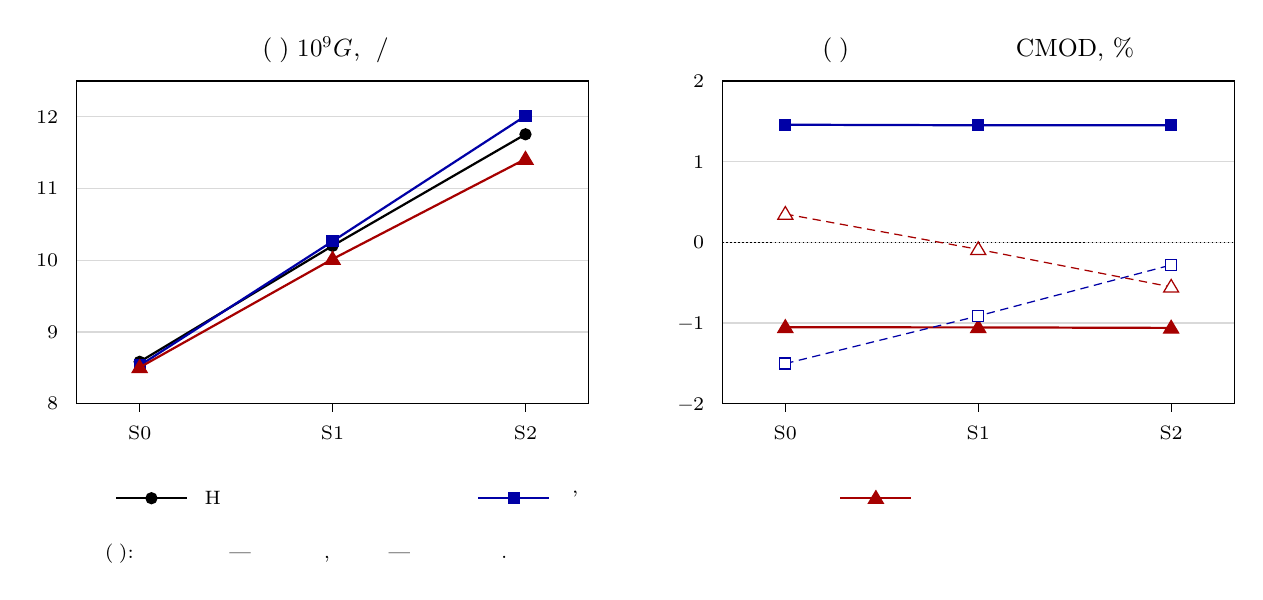
\begin{tikzpicture}[x=1mm,y=1mm,font=\small,line width=.45pt]
\draw[black!15] (0,0)--(65,0);\node[anchor=east,font=\scriptsize] at (-1,0) {$8$};
\draw[black!15] (0,9.1111)--(65,9.1111);\node[anchor=east,font=\scriptsize] at (-1,9.1111) {$9$};
\draw[black!15] (0,18.2222)--(65,18.2222);\node[anchor=east,font=\scriptsize] at (-1,18.2222) {$10$};
\draw[black!15] (0,27.3333)--(65,27.3333);\node[anchor=east,font=\scriptsize] at (-1,27.3333) {$11$};
\draw[black!15] (0,36.4444)--(65,36.4444);\node[anchor=east,font=\scriptsize] at (-1,36.4444) {$12$};
\draw (0,0) rectangle (65,41);\node[anchor=south] at (32.5,42) {(а) $10^9G$, Н/мм};
\draw (8,0)--(8,-1);\node[anchor=north,font=\scriptsize] at (8,-1.5) {S0};
\draw (32.5,0)--(32.5,-1);\node[anchor=north,font=\scriptsize] at (32.5,-1.5) {S1};
\draw (57,0)--(57,-1);\node[anchor=north,font=\scriptsize] at (57,-1.5) {S2};
\draw[black,line width=.8pt] (8,5.3261)--(32.5,20.0577)--(57,34.2187);
\draw[black,fill=black] (8,5.3261) circle[radius=.7mm];
\draw[black,fill=black] (32.5,20.0577) circle[radius=.7mm];
\draw[black,fill=black] (57,34.2187) circle[radius=.7mm];
\draw[blue!65!black,line width=.8pt] (8,4.8495)--(32.5,20.6338)--(57,36.5551);
\draw[blue!65!black,fill=blue!65!black] (7.3,4.1495) rectangle (8.7,5.5495);
\draw[blue!65!black,fill=blue!65!black] (31.8,19.9338) rectangle (33.2,21.3338);
\draw[blue!65!black,fill=blue!65!black] (56.3,35.8551) rectangle (57.7,37.2551);
\draw[red!65!black,line width=.8pt] (8,4.619)--(32.5,18.3726)--(57,31.0791);
\draw[red!65!black,fill=red!65!black] (8,5.569)--(7.05,3.969)--(8.95,3.969)--cycle;
\draw[red!65!black,fill=red!65!black] (32.5,19.3226)--(31.55,17.7226)--(33.45,17.7226)--cycle;
\draw[red!65!black,fill=red!65!black] (57,32.0291)--(56.05,30.4291)--(57.95,30.4291)--cycle;
\draw[black!15] (82,0)--(147,0);\node[anchor=east,font=\scriptsize] at (81,0) {$-2$};
\draw[black!15] (82,10.25)--(147,10.25);\node[anchor=east,font=\scriptsize] at (81,10.25) {$-1$};
\draw[black!15] (82,20.5)--(147,20.5);\node[anchor=east,font=\scriptsize] at (81,20.5) {$0$};
\draw[black!15] (82,30.75)--(147,30.75);\node[anchor=east,font=\scriptsize] at (81,30.75) {$1$};
\draw[black!15] (82,41)--(147,41);\node[anchor=east,font=\scriptsize] at (81,41) {$2$};
\draw[densely dotted] (82,20.5)--(147,20.5);
\draw (82,0) rectangle (147,41);\node[anchor=south] at (114.5,42) {(б) Зміна податливості та CMOD, \%};
\draw (90,0)--(90,-1);\node[anchor=north,font=\scriptsize] at (90,-1.5) {S0};
\draw (114.5,0)--(114.5,-1);\node[anchor=north,font=\scriptsize] at (114.5,-1.5) {S1};
\draw (139,0)--(139,-1);\node[anchor=north,font=\scriptsize] at (139,-1.5) {S2};
\draw[blue!65!black,line width=.8pt] (90,35.4344)--(114.5,35.3654)--(139,35.361);
\draw[blue!65!black,fill=blue!65!black] (89.3,34.7344) rectangle (90.7,36.1344);
\draw[blue!65!black,fill=blue!65!black] (113.8,34.6654) rectangle (115.2,36.0654);
\draw[blue!65!black,fill=blue!65!black] (138.3,34.661) rectangle (139.7,36.061);
\draw[red!65!black,line width=.8pt] (90,9.7081)--(114.5,9.6969)--(139,9.6302);
\draw[red!65!black,fill=red!65!black] (90,10.6581)--(89.05,9.0581)--(90.95,9.0581)--cycle;
\draw[red!65!black,fill=red!65!black] (114.5,10.6469)--(113.55,9.0469)--(115.45,9.0469)--cycle;
\draw[red!65!black,fill=red!65!black] (139,10.5802)--(138.05,8.9802)--(139.95,8.9802)--cycle;
\draw[blue!65!black,densely dashed] (90,5.0978)--(114.5,11.1473)--(139,17.6221);
\draw[blue!65!black,fill=white] (89.3,4.3978) rectangle (90.7,5.7978);
\draw[blue!65!black,fill=white] (113.8,10.4473) rectangle (115.2,11.8473);
\draw[blue!65!black,fill=white] (138.3,16.9221) rectangle (139.7,18.3221);
\draw[red!65!black,densely dashed] (90,24.0937)--(114.5,19.6071)--(139,14.8347);
\draw[red!65!black,fill=white] (90,25.0437)--(89.05,23.4437)--(90.95,23.4437)--cycle;
\draw[red!65!black,fill=white] (114.5,20.5571)--(113.55,18.9571)--(115.45,18.9571)--cycle;
\draw[red!65!black,fill=white] (139,15.7847)--(138.05,14.1847)--(139.95,14.1847)--cycle;
\draw[black,line width=.8pt] (5,-12)--(14,-12);
\draw[black,fill=black] (9.5,-12) circle[radius=.7mm];
\node[anchor=west,font=\scriptsize] at (15,-12) {H};
\draw[blue!65!black,line width=.8pt] (51,-12)--(60,-12);
\draw[blue!65!black,fill=blue!65!black] (54.8,-12.7) rectangle (56.2,-11.3);
\node[anchor=west,font=\scriptsize] at (61,-12) {М'які кільця};
\draw[red!65!black,line width=.8pt] (97,-12)--(106,-12);
\draw[red!65!black,fill=red!65!black] (101.5,-11.05)--(100.55,-12.65)--(102.45,-12.65)--cycle;
\node[anchor=west,font=\scriptsize] at (107,-12) {Жорсткі кільця};
\node[anchor=west,font=\scriptsize] at (0,-19) {На (б): суцільні лінії --- податливість, штрихові --- розкриття гирла.};
\end{tikzpicture}

 \caption{Абсолютне значення $G$ за сили 1 Н (а); відносні зміни податливості та нормального розкриття гирла тріщини (CMOD) відносно однорідної пластини (б).}
 \label{fig:fixed-structure}
\end{figure}

Розрахунки підтверджують передбачуваний знак зміни податливості: для м'яких кілець вона зростає приблизно на 1,45\,\%, для жорстких зменшується приблизно на 1,05\,\%. Ці контрасти майже однакові для трьох геометрій, хоча відповідні енергетичні контрасти істотно змінюються. Нормальне розкриття гирла також не відтворює закономірність зміни $G$: на S2 воно дещо зменшується для обох типів кілець. Отже, жодна з цих глобальних характеристик не є заміною КІН або $G$.

Окремо слід враховувати зміну опорного $G$ при подовженні тріщини. Для однорідної пластини $G$ зростає від $8{,}58457\cdot10^{-9}$ до $1{,}17557\cdot10^{-8}$ Н/мм (приблизно на 36,9\,\%). Абсолютне $G$ зростає також для обох неоднорідних конфігурацій. Від'ємний контраст означає меншу рушійну силу відносно однорідної пластини при тій самій довжині та геометрії, але не зменшення абсолютного $G$ зі збільшенням довжини. У цій задачі екранування не можна ототожнювати зі стабілізацією або зупинкою тріщини.

\section{Підсумок та перехід до вибіркового розташування кілець}
\label{sec:fixed-summary}

Перший розрахунковий експеримент дозволив встановити три закономірності в межах досліджених фіксованих геометрій. По-перше, знак прямого енергетичного ефекту м'яких кілець змінюється, тоді як знак напрямного ефекту зберігається. По-друге, після першого зламу зміна $G$ майже повністю визначається модою I, проте зміна напрямку залишається чутливою до моди II. По-третє, майже незмінний контраст податливості не визначає контрасту рушійної сили. Усі енергетичні ефекти ранньої серії розрізняються за первинним, але не за консервативним критерієм; на S2 додатково підтверджено стійкість до конкретної зміни зовнішньої сітки.

Водночас одночасна зміна жорсткості всіх трьох кілець не дозволяє встановити роль кожного кільця. Зокрема, від'ємний сумарний контраст не означає, що кожне з кілець окремо екранує тріщину. Це питання потребує розрахунків за вибіркової зміни матеріалу, з однаковою активною площею та незмінною геометрією. Йому присвячено наступний розділ. Питання зміни фактичної геометрії при незалежному чисельному розвитку тріщини розглянемо окремо.

\chapter{Вплив просторового розташування кілець та механізми зміни рушійної сили}
\label{ch:ring-placement}

У попередньому розділі встановлено, що одночасна зміна жорсткості трьох кілець може змінювати енергетичну рушійну силу та напрямок приросту тріщини по-різному. Проте сумарний ефект не дає інформації про роль окремих неоднорідностей. Зокрема, екранування тріщини трьома жорсткими кільцями не означає екранування кожним кільцем. У цьому розділі спочатку розглянемо вибіркову активацію кільцевих областей, потім дослідимо поля напружень та енергії деформації. Метою є не лише встановлення ефективніших архітектур, а й пояснення різних знаків їхнього впливу.

\section{Вибіркова зміна матеріальних характеристик}
\label{sec:ring-design}

Розглянемо зафіксовану однорідну геометрію S2 ($s=33{,}4$ мм). Координати вершини приблизно $(103{,}409;33{,}192)$ мм, кут локальної дотичної з віссю $x$ становить $76{,}45^\circ$. Позначимо через $\mathcal S\subseteq\{1,2,3\}$ множину активних кілець. Для спільного множника модуля $\lambda$ задаємо
\begin{equation}
 E_k=E_{\mathrm m}\begin{cases}
 \lambda,&k\in\mathcal S,\\
 1,&k\notin\mathcal S .
 \end{cases}
 \label{eq:ring-mask}
\end{equation}
Для кожного з двох значень $\lambda=0{,}5$ та 2 розглядаємо всі вісім підмножин, включно з порожньою. Отже, маємо 16 логічних випадків та 15 різних розподілів матеріальних характеристик: порожня множина відповідає одному й тому самому однорідному розв'язку. Вихідні однорідна конфігурація та дві конфігурації з усіма активними кільцями відтворюють попередню серію побітово; додатково обчислено 12 задач з неповними множинами. Геометрія, навантаження та сітка в усіх цих порівняннях однакові.

\begin{table}[htbp]
 \centering
 \caption{Положення кілець відносно вершини S2}
 \label{tab:ring-positions}
 \begin{tabular}{rrrrr}
 \toprule
 Кільце & $x_1$, мм & $x_2$, мм & Відстань, мм & Кут, град\\
 \midrule
 1 & 47,112 & $-39,042$ & 61,187 & $-39,649$\\
 2 & 96,499 & $-27,144$ & 100,244 & $-15,711$\\
 3 & 145,886 & $-15,246$ & 146,681 & $-5,966$\\
 \bottomrule
 \end{tabular}
\end{table}

У табл.~\ref{tab:ring-positions} координати центрів подано у локальному базисі вершини, кут відраховано від дотичної. Усі три центри лежать на одному боці від локальної осі тріщини, проте відстані та кути істотно різні. Дискретна площа кожного кільця однакова і становить $1012{,}152529$ мм$^2$. Тому порівняння трьох одиночних кілець при однаковому $\lambda$ є контрольованим дослідженням розташування за однакової кількості зміненого матеріалу. Необхідно водночас враховувати, що відстань, кут та положення відносно опор і сили змінюються разом; ця серія не відокремлює вплив кожного геометричного параметра.

\section{Енергетичні та напрямні ефекти однакової активної площі}
\label{sec:ring-results}

Позначимо через $F_G(\mathcal S;\lambda)$ контраст~\eqref{eq:problem-fixed-contrast}, а через $F_\theta(\mathcal S;\lambda)=\theta(\mathcal S;\lambda)-\theta_{\mathrm H}$ різницю локальних кутів МКН. Обидві величини дорівнюють нулю для порожньої множини. Результати наведено в табл.~\ref{tab:ring-results}; усі значення є прямими матеріальними ефектами на одній геометрії, а не результатами поширення тріщини.

\begin{table}[htbp]
 \centering
 \caption{Ефекти вибіркової активації кілець на S2}
 \label{tab:ring-results}
 \begin{tabular}{lrrrr}
 \toprule
 & \multicolumn{2}{c}{$F_G$, \%} & \multicolumn{2}{c}{$F_\theta$, град}\\
 \cmidrule(lr){2-3}\cmidrule(lr){4-5}
 $\mathcal S$ & $\lambda=0{,}5$ & $\lambda=2$ & $\lambda=0{,}5$ & $\lambda=2$\\
 \midrule
 $\varnothing$ & 0 & 0 & 0 & 0\\
$\{1\}$ & $4,430$ & $-3,652$ & $1,311$ & $-1,110$ \\
$\{2\}$ & $-3,628$ & $3,035$ & $-0,371$ & $0,306$ \\
$\{3\}$ & $2,331$ & $-1,825$ & $-0,353$ & $0,288$ \\
$\{1,2\}$ & $0,316$ & $-0,906$ & $1,058$ & $-0,734$ \\
$\{1,3\}$ & $6,747$ & $-5,478$ & $0,984$ & $-0,806$ \\
$\{2,3\}$ & $-1,675$ & $0,980$ & $-0,767$ & $0,574$ \\
$\{1,2,3\}$ & $2,181$ & $-2,931$ & $0,694$ & $-0,452$ \\
 \bottomrule
 \end{tabular}
\end{table}

\begin{figure}[htbp]
 \centering
 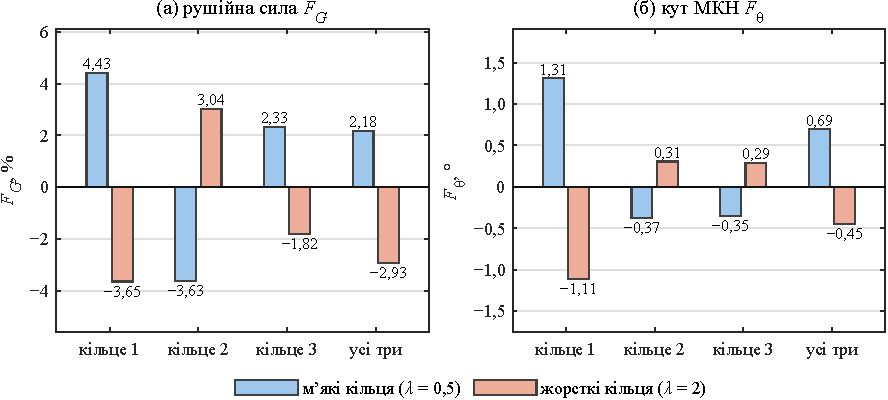
\includegraphics[width=\textwidth]{figures/F06_1_vnesky_kilets.pdf}
 \caption{Енергетичні та напрямні ефекти окремих кілець і одночасної активації всіх трьох кілець на фіксованій геометрії S2.}
 \label{fig:ring-single}
\end{figure}

Перший важливий результат полягає в тому, що кільце 2 впливає на $G$ протилежно до кілець 1 і 3. Пом'якшення кільця 1 збільшує $G$ на 4,43\,\%, тоді як пом'якшення кільця 2 зменшує його на 3,63\,\%. Різниця становить 8,06 відсоткового пункта за однакових модулів і активної площі. Ця різниця розрізняється за обома прийнятими критеріями. Вплив третього кільця за модулем менший, проте його знак збігається зі знаком першого. Для жорстких кілець знаки всіх трьох ефектів протилежні відповідним ефектам м'яких кілець. Водночас за консервативним критерієм енергетичні ефекти жорсткого кільця 2 та третього кільця при обох контрастах залишаються нерозрізненими.

Віддаленість сама по собі не визначає знака ефекту. За модулем одиночні енергетичні ефекти в цій серії справді впорядковуються відповідно до відстані: $|F_G(\{1\})|>|F_G(\{2\})|>|F_G(\{3\})|$. Проте навіть третє кільце, центр якого віддалений приблизно на 147 мм, дає обчислений контраст порядку двох відсотків. Залежність знака від розташування є істотною особливістю задачі, яка не випливає з простої оцінки затухання локального збурення біля тріщини.

Для кута МКН інша група знаків: кільце 1 має протилежний напрямний ефект до кілець 2 і 3. Найближче кільце змінює кут у 3,5--3,9 раза сильніше, ніж кожне з двох інших. Таким чином, групування кілець за знаком енергетичного ефекту не збігається з групуванням за знаком напрямного. Це узгоджується з розмежуванням модових чутливостей у підрозділі~\ref{sec:fixed-steering}.

\begin{figure}[htbp]
 \centering
 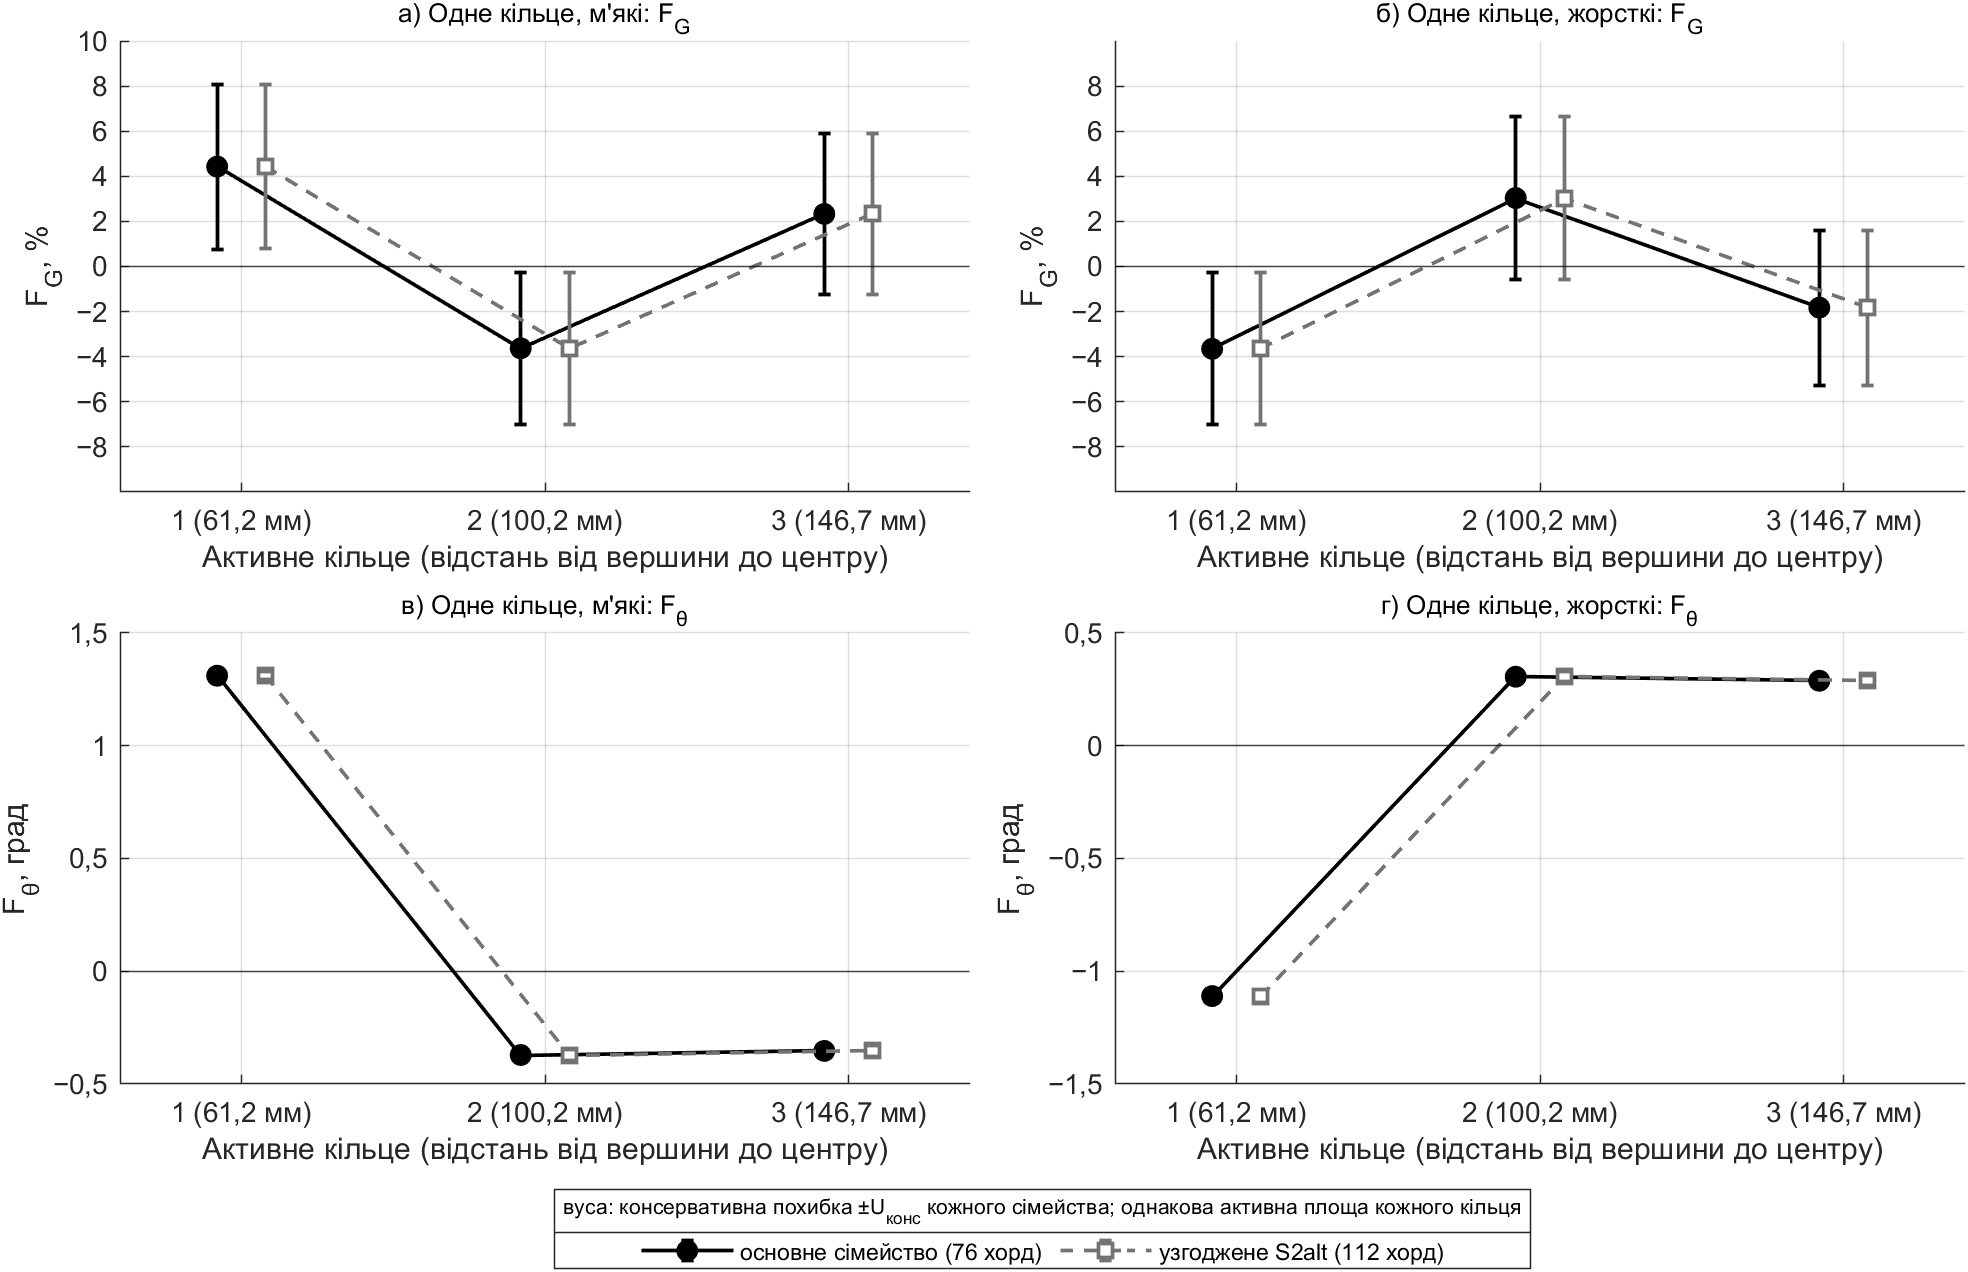
\includegraphics[width=\textwidth]{figures/r1_g3_equal_area_grey.png}
 \caption{Ефекти одиночних кілець при однаковій активній площі: порівняння вихідної та альтернативної зовнішніх сіток на S2.}
 \label{fig:ring-equal-area}
\end{figure}

Порівняння R1 підтвердило стійкість усіх шести одиночних енергетичних і шести кутових контрастів до конкретної заміни зовнішньої сітки. Збережено також усі чотири порядки ранжування (два контрасти жорсткості та дві характеристики). Детальні чисельні показники наведено в підрозділі~\ref{sec:ver-exterior}. Не слід переносити це приймання на всі комбінації: на альтернативній сітці з двокільцевих варіантів розглянуто лише жорстку пару $\{1,3\}$.

Друга важлива закономірність стосується комбінацій. За однакової площі двох жорстких кілець контрасти для $\{1,2\}$, $\{1,3\}$ та $\{2,3\}$ становлять відповідно $-0{,}906$, $-5{,}478$ та $+0{,}980$\,\%. Отже, збільшення кількості жорсткого матеріалу не гарантує зменшення $G$. Найменше $G$ серед розглянутих конфігурацій отримано для жорсткої пари $\{1,3\}$, а найбільше --- для м'якої пари $\{1,3\}$. Це не глобальна оптимізація: не змінювалися радіуси, координати кілець, змішані контрасти або схема навантаження.

\begin{figure}[htbp]
 \centering
 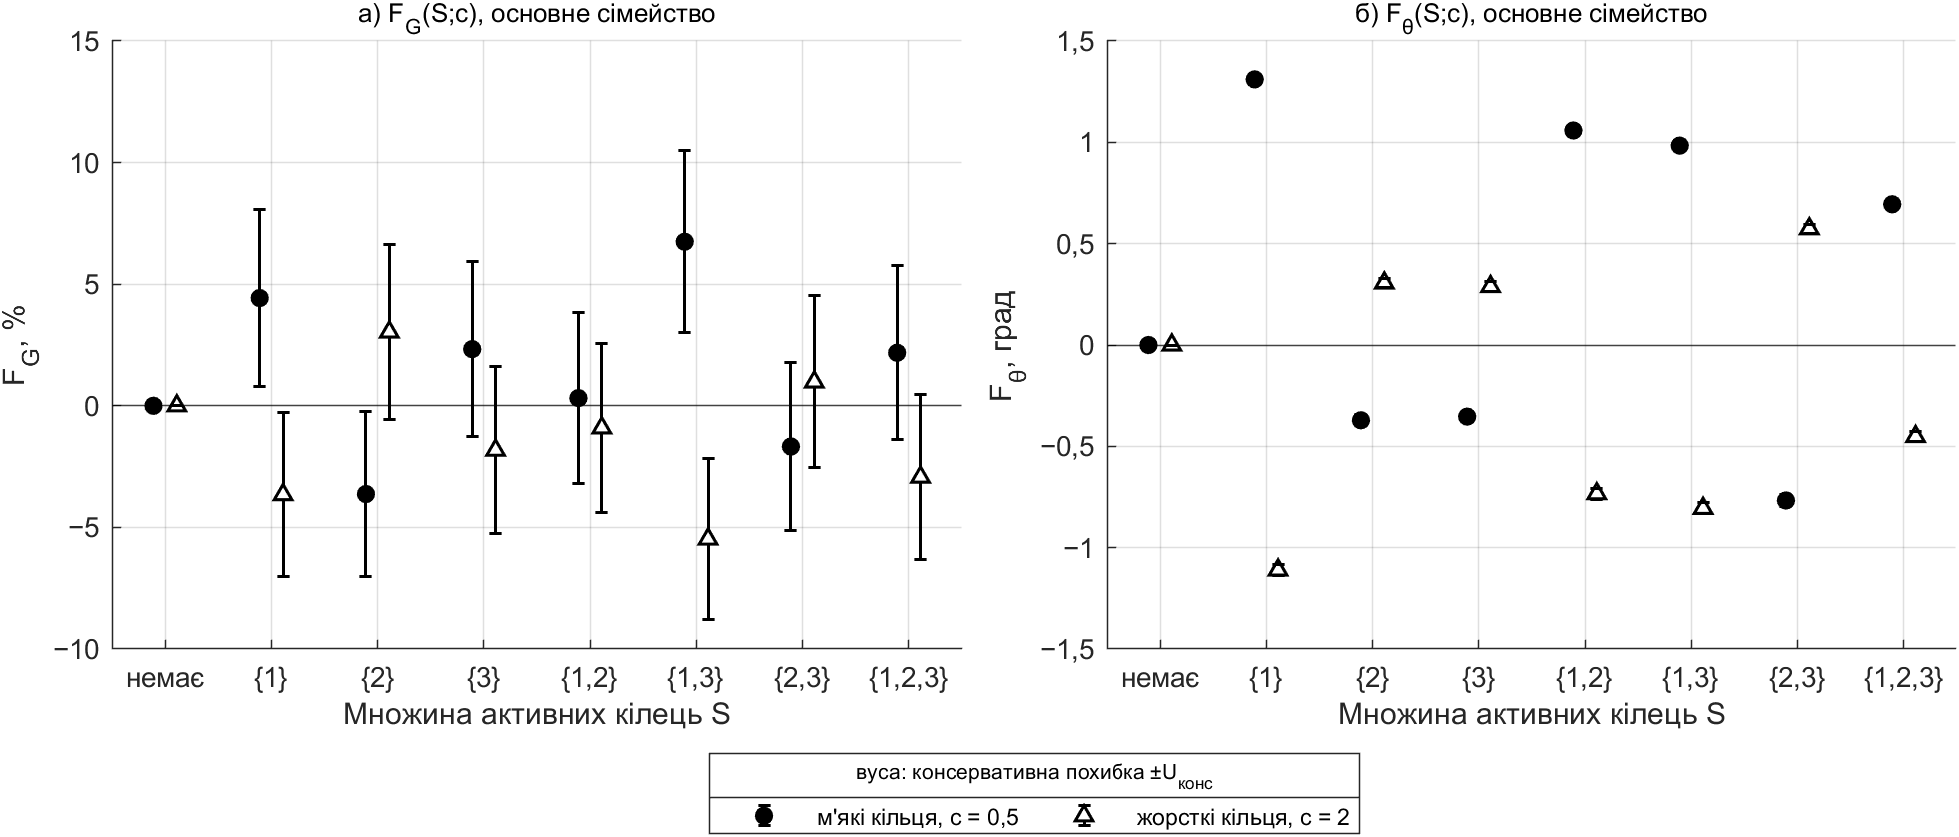
\includegraphics[width=\textwidth]{figures/r1_g6_m4b_masks_grey.png}
 \caption{Енергетичні й напрямні характеристики конфігурацій з різними множинами активних кілець на вихідній сітці S2.}
 \label{fig:ring-masks}
\end{figure}

\section{Адитивність і взаємодія матеріальних неоднорідностей}
\label{sec:ring-nonadditive}

Чи можна оцінити сумарний вплив декількох кілець, підсумовуючи ефекти одиночних? Для довільної характеристики $F$ (далі $F_G$ або $F_\theta$) і фіксованого контрасту $\lambda$ введемо
\begin{equation}
 f_i=F(\{i\}),\qquad
 I_{ij}=F(\{i,j\})-f_i-f_j.
 \label{eq:ring-pair}
\end{equation}
Внесок потрійної взаємодії визначимо як
\begin{equation}
 I_{123}=F(\{1,2,3\})-\sum_i f_i-\sum_{i<j}I_{ij}.
 \label{eq:ring-triple}
\end{equation}
Тоді точна тотожність
\begin{equation}
 F(\{1,2,3\})=\sum_i f_i+\sum_{i<j}I_{ij}+I_{123}
 \label{eq:ring-reconstruct}
\end{equation}
є розкладом функції множини за включенням і виключенням. Він не передбачає фізичної лінійності щодо контрасту жорсткості. Зокрема, лінійність крайової задачі за навантаженням не означає лінійності розв'язку за матрицею жорсткості. Крім того, $G$ є квадратичною, а кут МКН --- нелінійною функцією КІН. Ненульові $I$ можуть відображати обидві ці обставини; без додаткового розкладу їх не можна ототожнювати тільки з просторовою взаємодією полів.

Для симетричного розподілу сумарного ефекту між окремими кільцями використовуємо також величини Шеплі:
\begin{equation}
 \phi_i=f_i+\frac12\sum_{j\ne i}I_{ij}+\frac13 I_{123},
 \qquad \sum_i\phi_i=F(\{1,2,3\}).
 \label{eq:ring-shapley}
\end{equation}
Це середній граничний внесок кільця при всіх порядках його додавання. Величини $\phi_i$ не є незалежними фізичними енергіями і відрізняються від ефектів одиночних кілець.

\begin{table}[htbp]
 \centering
 \caption{Розклад енергетичних і кутових контрастів на S2. Зірочка означає розрізнення за обома критеріями; інші наведені внески розрізняються лише за первинним.}
 \label{tab:ring-decomp}
 \begin{tabular}{lrrrr}
 \toprule
 & \multicolumn{2}{c}{$F_G$, \%} & \multicolumn{2}{c}{$F_\theta$, град}\\
 \cmidrule(lr){2-3}\cmidrule(lr){4-5}
 Внесок & $\lambda=0{,}5$ & $\lambda=2$ & $\lambda=0{,}5$ & $\lambda=2$\\
 \midrule
$f_{1}$ & $4,4298^{*}$ & $-3,6517^{*}$ & $1,3106^{*}$ & $-1,1100^{*}$ \\
$f_{2}$ & $-3,6278^{*}$ & $3,0352$ & $-0,3714^{*}$ & $0,3061^{*}$ \\
$f_{3}$ & $2,3310$ & $-1,8248$ & $-0,3534^{*}$ & $0,2883^{*}$ \\
$I_{12}$ & $-0,4861$ & $-0,2893$ & $0,1192^{*}$ & $0,0703^{*}$ \\
$I_{13}$ & $-0,0143$ & $-0,0014$ & $0,0264$ & $0,0158$ \\
$I_{23}$ & $-0,3780$ & $-0,2301$ & $-0,0424$ & $-0,0207$ \\
$I_{123}$ & $-0,0733$ & $0,0309$ & $0,0054$ & $-0,0014$ \\
$\phi_{1}$ & $4,1552^{*}$ & $-3,7868^{*}$ & $1,3852^{*}$ & $-1,0674^{*}$ \\
$\phi_{2}$ & $-4,0843^{*}$ & $2,7858$ & $-0,3313^{*}$ & $0,3304^{*}$ \\
$\phi_{3}$ & $2,1105$ & $-1,9303$ & $-0,3596^{*}$ & $0,2854^{*}$ \\
 \bottomrule
 \end{tabular}
\end{table}

\begin{figure}[htbp]
 \centering
 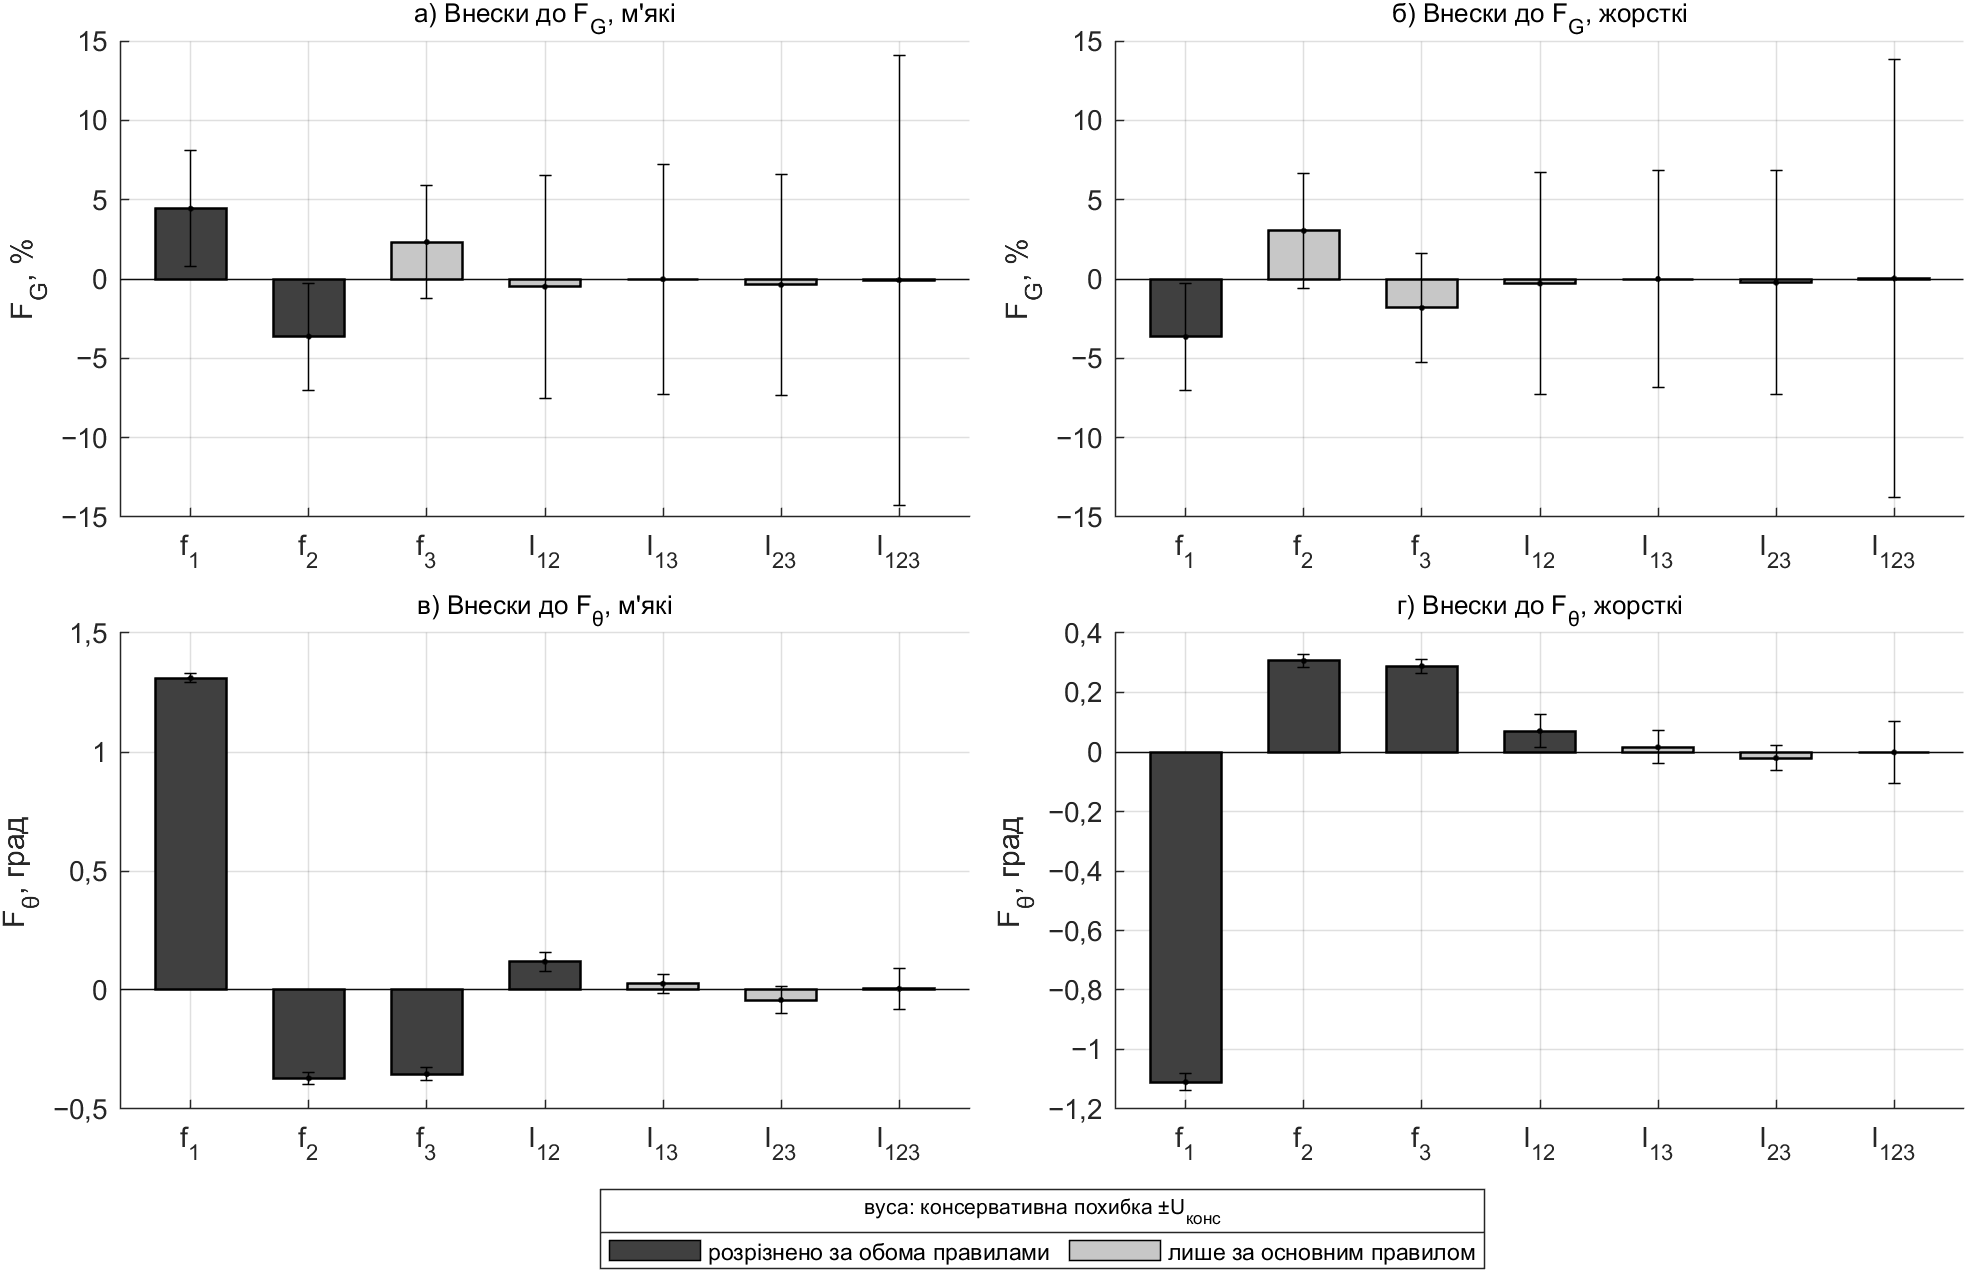
\includegraphics[width=\textwidth]{figures/r1_g7_m4b_decomposition_grey.png}
 \caption{Основні внески та взаємодії матеріальних неоднорідностей; розрізнення за первинним і консервативним критеріями.}
 \label{fig:ring-decomp}
\end{figure}

Для трьох м'яких кілець сума одиночних ефектів становить приблизно $+3{,}133$\,\%, а сумарний ефект --- $+2{,}181$\,\%. Різниця близько $-0{,}952$ відсоткового пункта складається з усіх взаємодій. Для жорстких кілець відповідні величини $-2{,}441$ та $-2{,}931$\,\%. Найбільші парні енергетичні взаємодії за модулем не перевищують 0,49 відсоткового пункта; вони менші за основні ефекти, але можуть бути істотними при взаємному компенсуванні останніх.

Усі енергетичні взаємодії розрізняються за первинним критерієм, однак жодна --- за консервативним. Особливо мала взаємодія $I_{13}$ для жорстких кілець (близько $-1{,}44\cdot10^{-5}$ у безрозмірних одиницях) має порядок спостереженої міжсіткової зміни одиночних контрастів. Не слід приписувати її знаку фізичний зміст. Незалежне повторення всього розкладу на іншій сітці не виконано. Для кута МКН взаємодія $I_{12}$ розрізняється за обома критеріями при обох контрастах; інші взаємодії --- лише за первинним.

Таким чином, просте підсумовування одиночних внесків є наближенням, а не точною властивістю матеріальної архітектури. Вибір конфігурацій для подальшого дослідження має враховувати не тільки знак одиночного ефекту, а й можливе компенсування внесків.

\section{Поля напружень та енергії деформації}
\label{sec:ring-fields}

Для пояснення результатів відновлено напруження, деформації та густину енергії
\begin{equation}
 w(\boldsymbol x)=\tfrac12\boldsymbol\sigma(\boldsymbol x):
 \boldsymbol\varepsilon(\boldsymbol x)
 \label{eq:ring-w}
\end{equation}
зі збережених переміщень T6 для однорідного стану та шести одиночних кілець на двох сітках. Енергії елементів, обчислені триточковою квадратурою, збігаються зі збереженими до $1{,}9\cdot10^{-13}$ у відносних одиницях. Це перевірка відтворення поля, а не експериментальна валідація.

\begin{figure}[htbp]
 \centering
 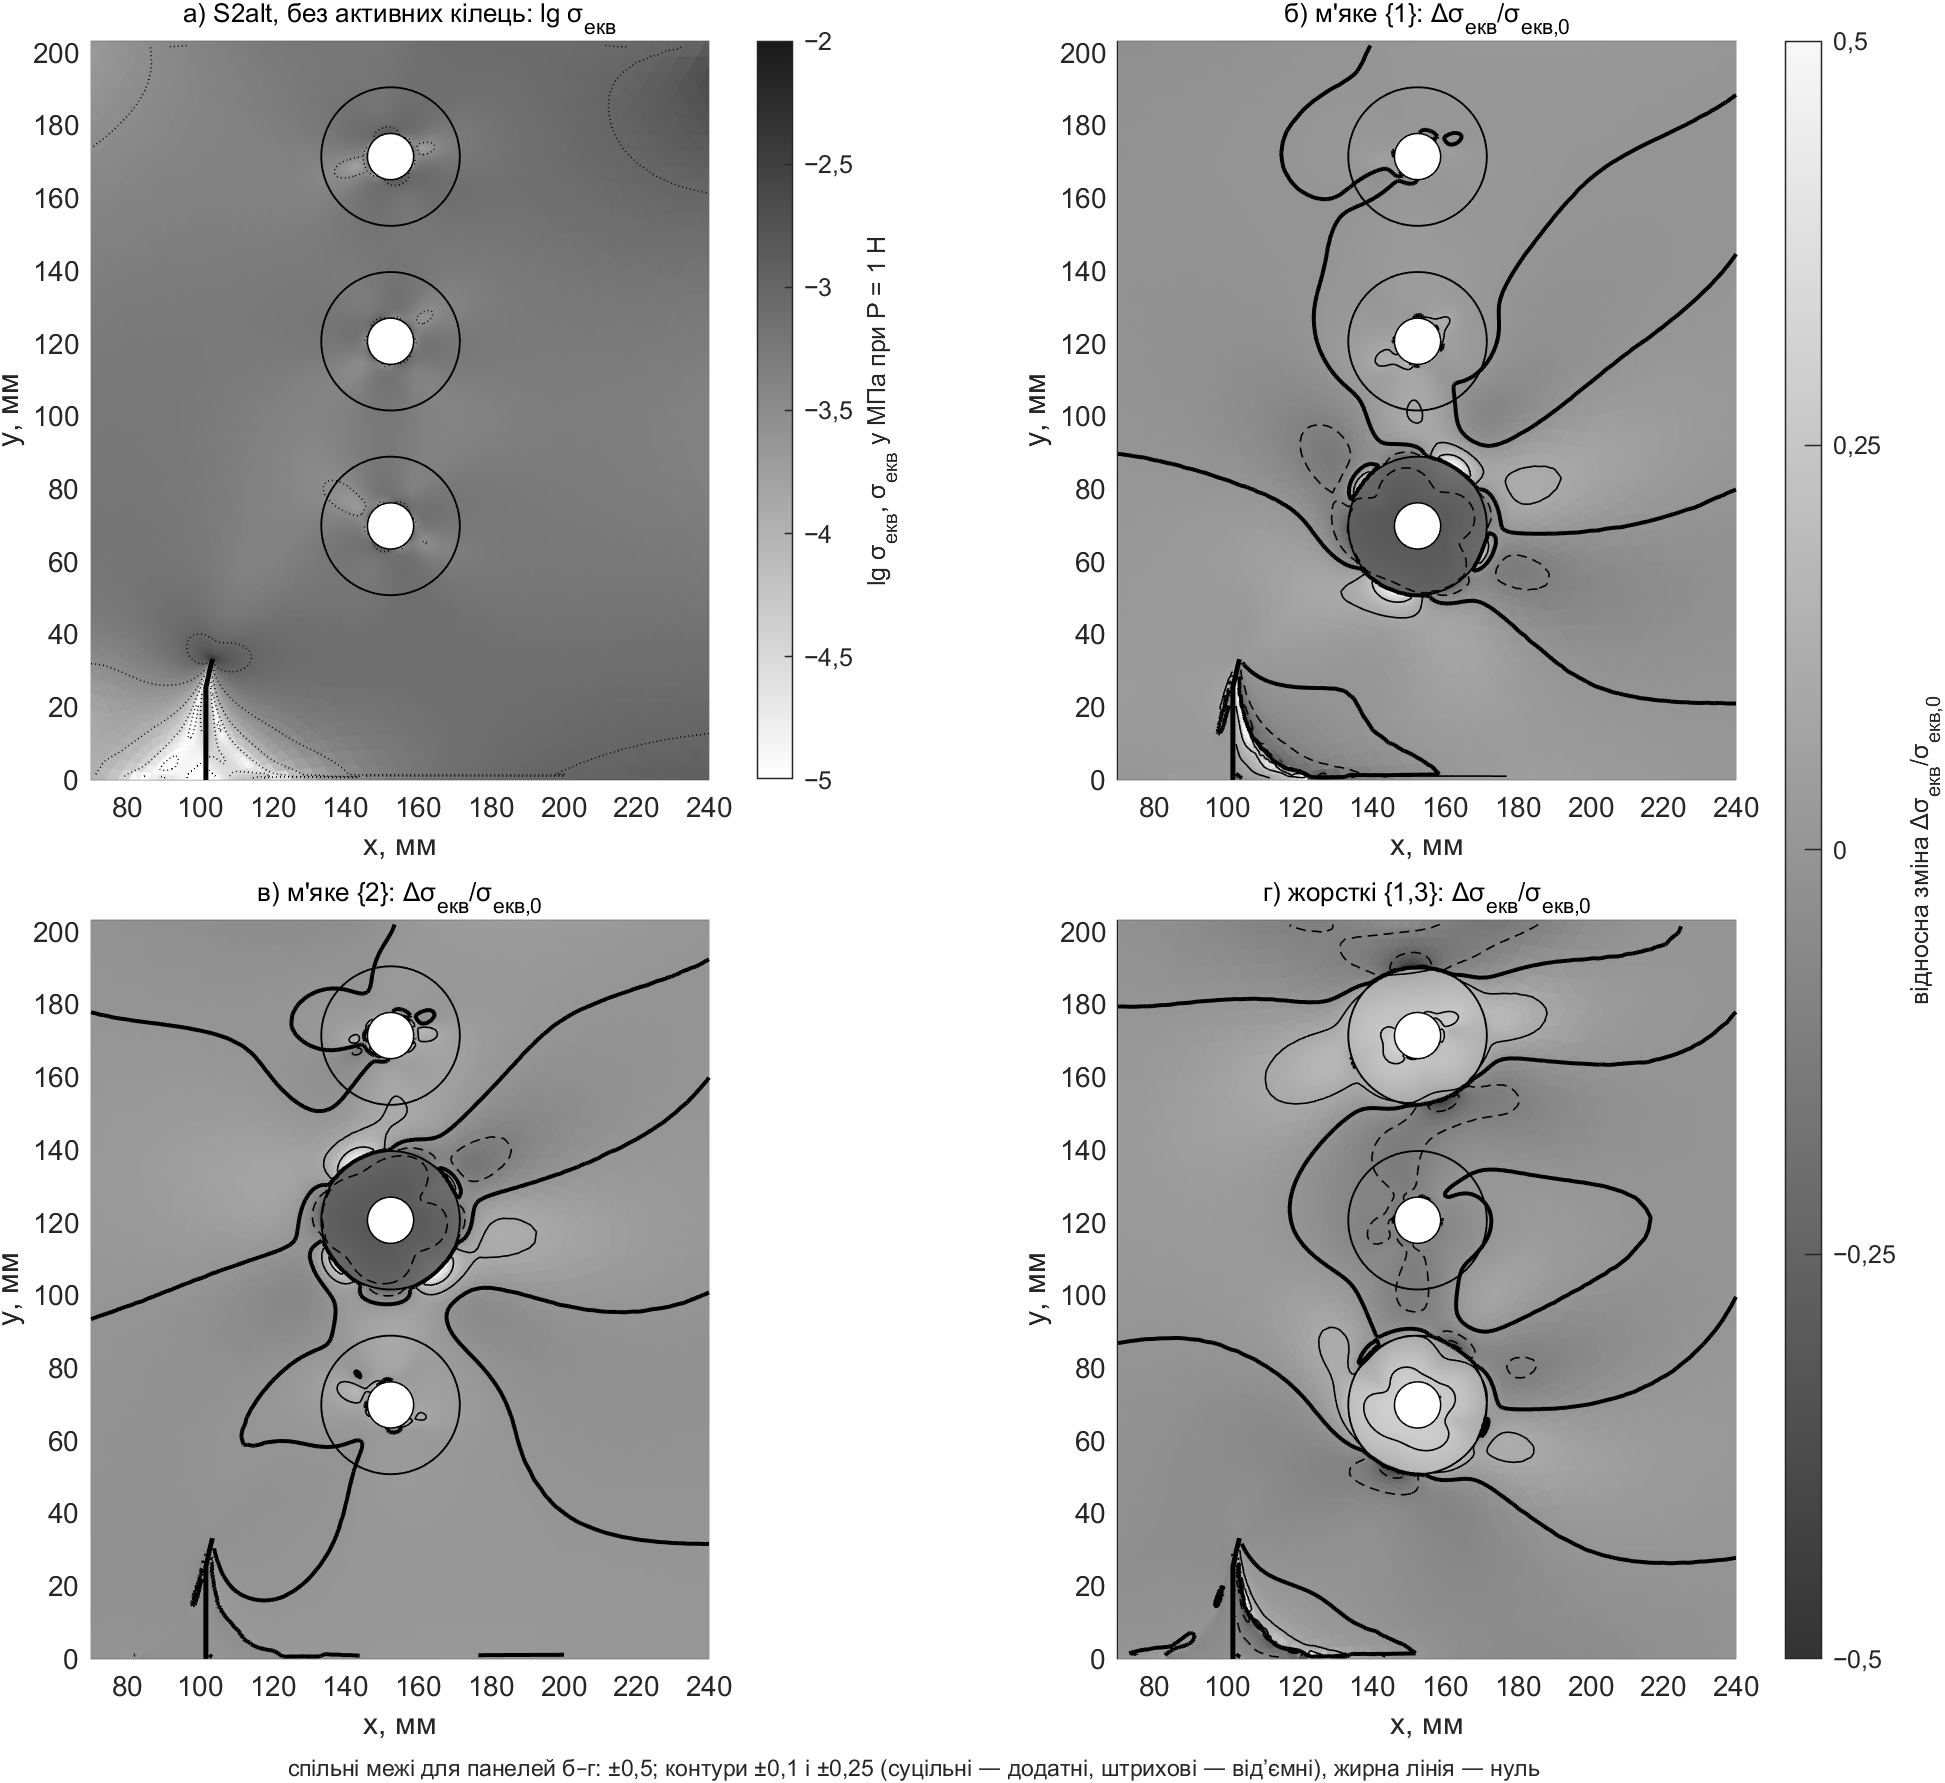
\includegraphics[width=\textwidth]{figures/r1_g4_stress_global_grey.png}
 \caption{Еквівалентні напруження однорідної пластини та відносна зміна поля для вибраних архітектур на альтернативній сітці S2. Для відносних змін використано спільну шкалу.}
 \label{fig:ring-von-mises}
\end{figure}

\begin{figure}[htbp]
 \centering
 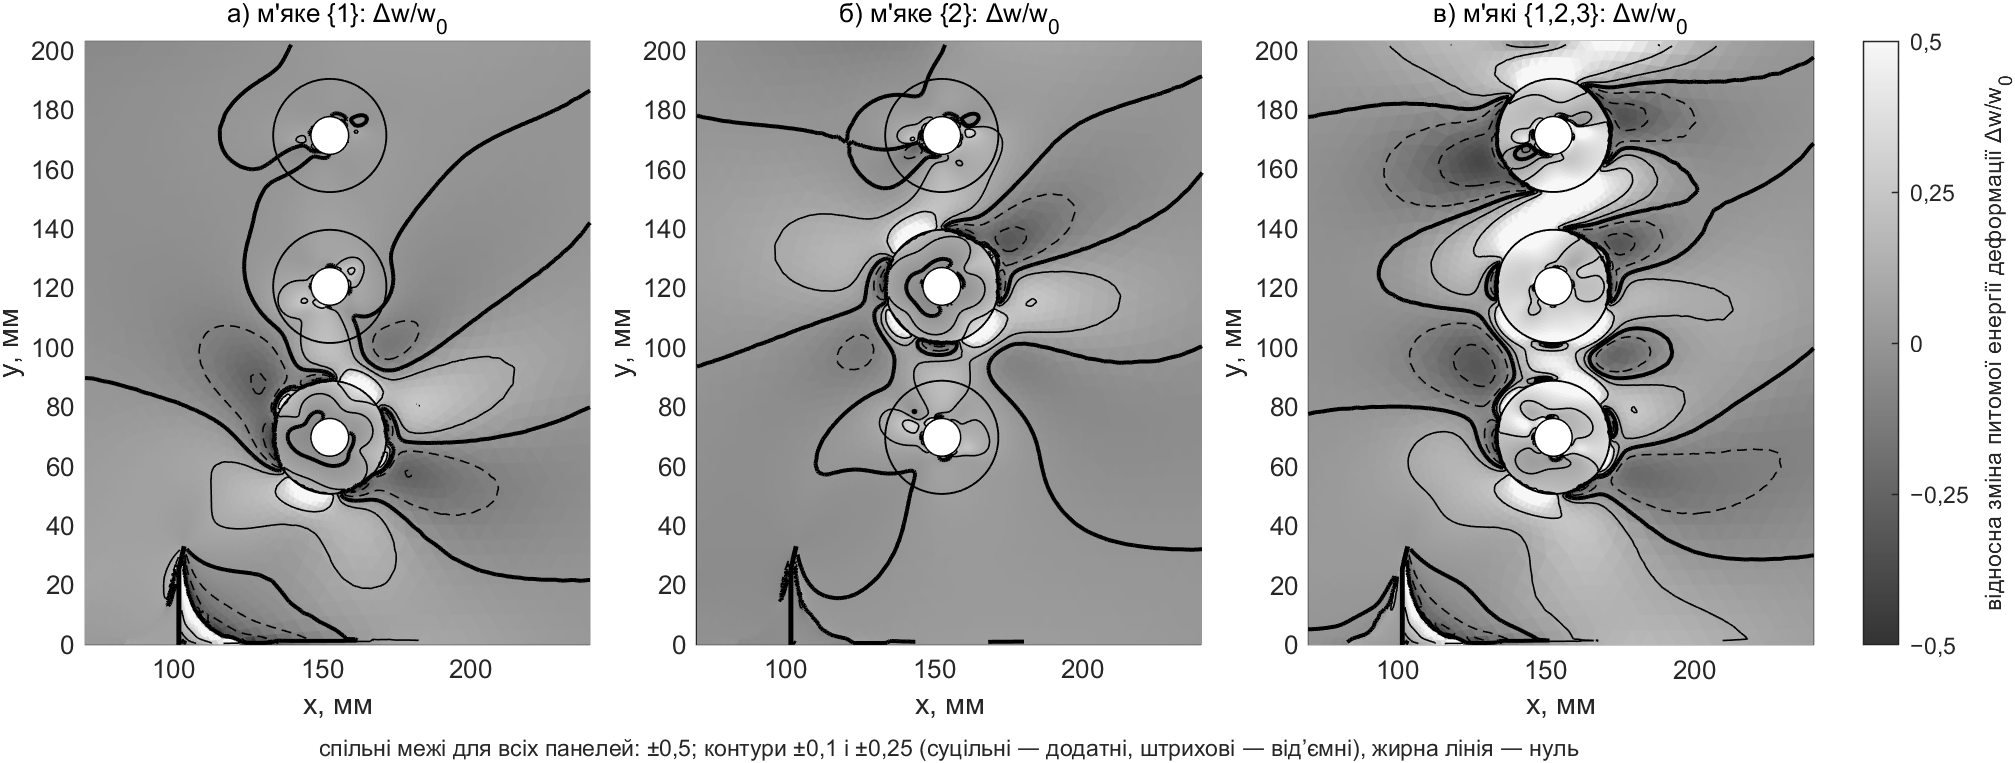
\includegraphics[width=\textwidth]{figures/r1_g5_energy_density_grey.png}
 \caption{Відносна зміна середньої по елементах густини енергії деформації для вибраних м'яких кілець на вихідній сітці S2; спільна шкала відносних змін.}
 \label{fig:ring-energy-maps}
\end{figure}

Карти еквівалентного напруження показують, що м'які кільця зменшують напруження в активованих областях, тоді як жорсткі збільшують їх. Для розглянутих м'яких кілець медіанне зменшення еквівалентного напруження в активній області становить близько 29\,\%; для жорсткої пари зростання в кільцях 1 і 3 становить приблизно 26 та 22\,\%. При цьому медіанна зміна в матриці мала, але просторове збурення простежується далеко від активної області. Карти енергії (рис.~\ref{fig:ring-energy-maps}) також показують перерозподіл по навантаженій частині пластини. Ці відомості не встановлюють знак зміни $G$: для цього потрібно дослідити зміну поля при варіації геометрії тріщини.

\subsection{Гіпотеза про передачу навантаження від сили до опори}

Пряма між лівою опорою та точкою прикладання сили проходить на відстані 5,8 мм від центра кільця 2. Центри кілець 1 і 3 розташовані по різні боки від неї (відповідні знакові відстані $-32{,}2$ та $+43{,}8$ мм). Виникає гіпотеза, що кільце 2 належить до особливої області передачі навантаження і тому його вплив протилежний впливу двох інших кілець. Перевіримо, чи є ця пряма траєкторією головного стиску або областю концентрації енергії.

\begin{figure}[htbp]
 \centering
 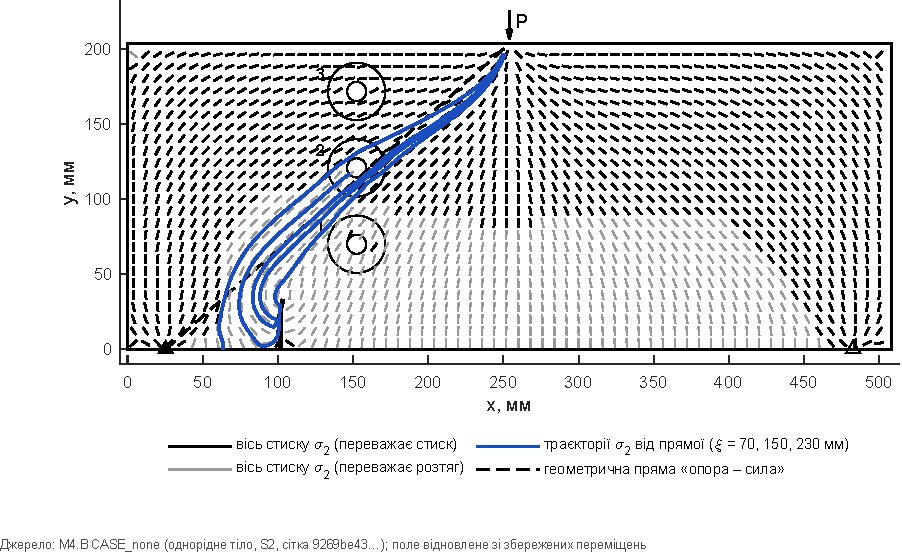
\includegraphics[width=\textwidth]{figures/G1_1_napriamy_stysku_UA.pdf}
 \caption{Осі меншого головного напруження та наближені траєкторії цих осей у однорідній пластині S2. Пряму між лівою опорою і силою використано як геометричний орієнтир.}
 \label{fig:ring-principal}
\end{figure}

\begin{figure}[htbp]
 \centering
 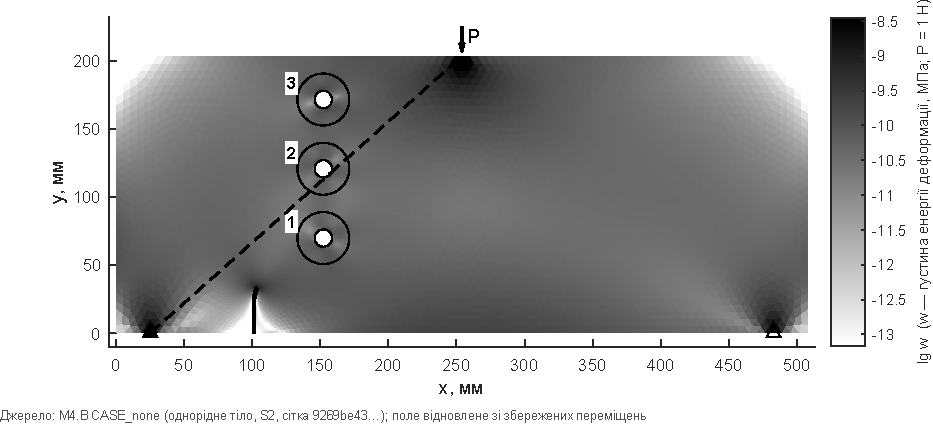
\includegraphics[width=\textwidth]{figures/G1_2_gustyna_energii_UA.pdf}
 \caption{Густина енергії деформації однорідної пластини S2 (логарифмічна шкала, сила 1 Н). Поле відновлено зі збережених переміщень.}
 \label{fig:ring-w-reference}
\end{figure}

У смузі півшириною 10 мм навколо прямої медіанне відхилення осі стиску від напряму прямої дорівнює $11{,}4^\circ$; приблизно 61\,\% площі має відхилення не більше $15^\circ$. У двох паралельних смугах зі зміщеннями $\pm30$ мм відповідні медіанні кути становлять $16{,}1^\circ$ та $14{,}8^\circ$. Уздовж верхньої частини прямої траєкторії осей стиску відхиляються від неї не більше ніж приблизно на 10 мм; нижче отвору 2 відхилення досягають 26--44 мм, і жодна з досліджених ліній не досягає лівої опори. Ці лінії відновлено чисельно з центроїдних напрямків елементів, тому вони є наближеними траєкторіями, а не точними характеристиками неперервного поля.

Області найбільших стискальних напружень не збігаються з прямою. У кількох поперечних перерізах їхні екстремуми розташовані на 38--52 мм вище неї. Середні густини енергії в центральній та зміщеній на 30 мм смугах майже однакові ($5{,}63\cdot10^{-11}$ та $5{,}69\cdot10^{-11}$ МПа). Таким чином, пряму не можна вважати ні повною траєкторією головних напружень, ні гребенем стиску чи енергії.

\begin{table}[htbp]
 \centering
 \caption{Напружений стан областей кілець в однорідній пластині S2. Головні напруження усередненого тензора наведено в одиницях $10^{-4}$ МПа при $P=1$ Н.}
 \label{tab:ring-stress}
 \begin{tabular}{rrrrrr}
 \toprule
 Кільце & Відстань, мм & $\sigma_1$ & $\sigma_2$ & Кут, град & Стиск, \%\\
 \midrule
 1 & $-32,2$ & $+4,24$ & $-1,59$ & 21,1 & 12\\
 2 & $+5,8$ & $+1,92$ & $-3,81$ & 5,1 & 75\\
 3 & $+43,8$ & $+0,50$ & $-5,72$ & 27,1 & 96\\
 \bottomrule
 \end{tabular}
\end{table}

У табл.~\ref{tab:ring-stress} наведено власні значення усередненого по кільцю тензора, кут його осі стиску відносно прямої та частку площі, на якій стиск домінує за модулем головних напружень. Ця частка не є часткою двовісно стиснутого матеріалу. Зокрема, для кільця 2 $\sigma_1>0$, а $\sigma_2<0$; отже, усереднений стан має одночасно розтягальне та стискальне головні напруження з переважанням стиску. У кільці 1 переважає розтяг, у кільці 3 --- стиск. Попри це, кільця 1 і 3 мають однакові знаки енергетичних ефектів. Сам тип напруженого стану не визначає знак впливу на $G$.

\begin{figure}[htbp]
 \centering
 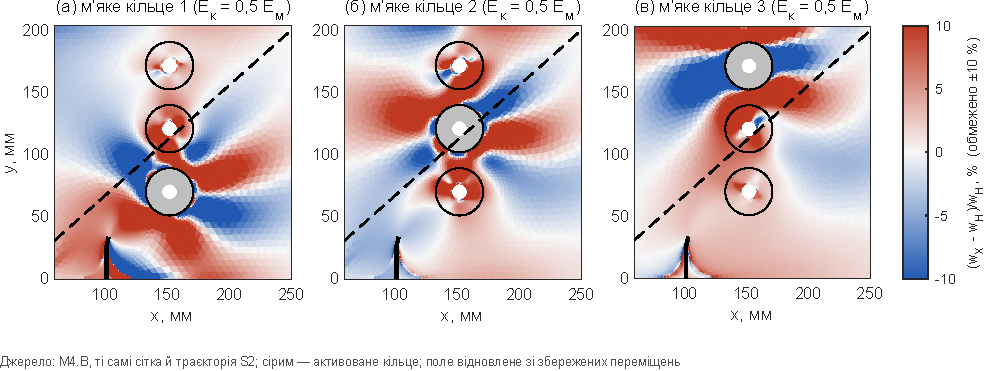
\includegraphics[width=\textwidth]{figures/G1_3_pererozpodil_energii_UA.pdf}
 \caption{Відносна зміна густини енергії поза активованим м'яким кільцем: (а) кільце 1, (б) кільце 2, (в) кільце 3. Активну область замасковано; шкала обмежена інтервалом від $-10$ до $+10$ відсотків.}
 \label{fig:ring-single-fields}
\end{figure}

Активація м'яких кілець створює області зменшення та збільшення густини енергії поза самими кільцями (рис.~\ref{fig:ring-single-fields}). Для кільця 2 область зменшення витягнута приблизно вздовж прямої опора--сила. Для інших кілець її орієнтація відрізняється. Проте просторовий розподіл $w_X-w_{\mathrm H}$ при фіксованій тріщині не є сам по собі полем чутливості $G$ до матеріального контрасту.

\section{Енергетична чутливість до локальної зміни матеріалу}
\label{sec:ring-sensitivity}

\subsection{Варіаційне обґрунтування}

Розглянемо фіксовану геометрію, лінійно-пружну систему під заданим навантаженням $P$. Нехай $\boldsymbol S$ --- тензор пружної податливості матеріалу, а $\boldsymbol S_{\mathrm H}$ --- його значення в однорідній матриці. За однакового коефіцієнта Пуассона зміна модуля в кільці $k$ еквівалентна
\begin{equation}
 \boldsymbol S_X-\boldsymbol S_{\mathrm H}
 =\eta_k\boldsymbol S_{\mathrm H},\qquad
 \eta_k=\lambda_k^{-1}-1,\quad \boldsymbol x\in\Omega_k .
 \label{eq:ring-eta}
\end{equation}
Поза активними кільцями ця різниця нульова. Для двох рівноважних полів на тій самій геометрії та при тих самих силах принцип віртуальних робіт дає
\begin{equation}
 \begin{aligned}
 P^2 C_X &=t\int_\Omega \boldsymbol\sigma_{\mathrm H}:
                     \boldsymbol\varepsilon_X\,\mathrm d\Omega,\\
 P^2 C_{\mathrm H}&=t\int_\Omega \boldsymbol\sigma_X:
                     \boldsymbol\varepsilon_{\mathrm H}\,\mathrm d\Omega .
 \end{aligned}
 \label{eq:ring-betti-works}
\end{equation}
Використовуючи симетрію тензорів податливості, отримаємо точну перехресну тотожність
\begin{equation}
 C_X-C_{\mathrm H}=\frac{t}{P^2}\sum_k\eta_k
 \int_{\Omega_k}
 \boldsymbol\sigma_{\mathrm H}:\boldsymbol S_{\mathrm H}:
 \boldsymbol\sigma_X\,\mathrm d\Omega .
 \label{eq:ring-betti}
\end{equation}
Вона справедлива також для дискретних полів на спільній узгодженій сітці при точному збиранні білінійних форм. Для 12 одиночних випадків (дві сітки) перехресний інтеграл відтворив записану зміну податливості; максимальна повідомлена розбіжність не перевищує $1{,}9\cdot10^{-10}$ за показником вихідного аудиту.

За малого контрасту та регулярної залежності розв'язку від матеріальних параметрів $\boldsymbol\sigma_X=\boldsymbol\sigma_{\mathrm H}+O(\|\boldsymbol\eta\|)$ у відповідній енергетичній нормі. Позначимо енергію однорідного тіла в області $k$ та повну енергію, віднесені до одиниці товщини, через
\begin{equation}
 \mathcal W_k^{\mathrm H}=\int_{\Omega_k} w_{\mathrm H}\,\mathrm d\Omega,
 \qquad \mathcal W_{\mathrm H}=\int_\Omega w_{\mathrm H}\,\mathrm d\Omega .
 \label{eq:ring-energies}
\end{equation}
Повна енергія дорівнює $t\mathcal W=P^2 C/2$. Із~\eqref{eq:ring-betti} випливає
\begin{equation}
 \mathcal W_X-\mathcal W_{\mathrm H}
 =\sum_k\eta_k\mathcal W_k^{\mathrm H}
 +O(\|\boldsymbol\eta\|^2).
 \label{eq:ring-first-energy}
\end{equation}
Це також є наслідком стаціонарності доповнювальної енергії: в першому порядку для варіації податливості достатньо однорідного поля. Розклад стосується енергії всієї конструкції, а не припущення про незмінність напружень у кільці за скінченного контрасту.

Якщо похідну за довжиною $s$ розуміти як похідну форми при одному й тому самому віртуальному прирості тріщини, то за силового навантаження $G=\partial_s\mathcal W$ (див.~\eqref{eq:fixed-compliance-G}). За достатньої гладкості змішаної чутливості з~\eqref{eq:ring-first-energy} отримуємо
\begin{equation}
 \left.\frac{\partial G}{\partial\eta_k}\right|_{\boldsymbol\eta=0}
 =\partial_s\mathcal W_k^{\mathrm H},
 \qquad
 F_G^{(1)}=\sum_k\eta_k
 \frac{\partial_s\mathcal W_k^{\mathrm H}}{\partial_s\mathcal W_{\mathrm H}}.
 \label{eq:ring-first-G}
\end{equation}
Отже, знак першого порядку визначає не сама густина енергії і не знак головного напруження, а похідна енергії в області майбутньої неоднорідності за геометричним приростом тріщини. Якщо ця область розвантажується при рості тріщини, то її пом'якшення у першому порядку зменшує $G$. Якщо довантажується, пом'якшення збільшує $G$.

Слід розрізняти точну похідну форми та її чисельне наближення різницями енергій уздовж ламаної однорідної траєкторії. В останньому випадку змінюються сітка і напрямок приросту, а точкове навантаження створює додаткову сіткову залежність енергії. Тому далі перевіряємо саме наближення~\eqref{eq:ring-first-G}, а не точну похідну форми. Для скінченних контрастів $\eta=1$ та $-0{,}5$ немає підстав вважати члени вищих порядків малими без додаткового дослідження.

\subsection{Зміна енергії в областях кілець уздовж однорідної траєкторії}

Використаємо збережені однорідні стани S0--S4. На цьому етапі матеріал усіх кілець збігається з матрицею, а їхні контури визначають області інтегрування. Енергії наведено в табл.~\ref{tab:ring-energies}. Відносні зміни в кільцях на порядок більші за відносну зміну повної енергії.

\begin{table}[htbp]
 \centering
 \caption{Енергії на одиницю товщини, Н: $\mathcal W_k$ в одиницях $10^{-8}$ Н; $\mathcal W_{\mathrm H}$ в одиницях $10^{-6}$ Н.}
 \label{tab:ring-energies}
 \begin{tabular}{lrrrr}
 \toprule
 Стан & $\mathcal W_1$ & $\mathcal W_2$ & $\mathcal W_3$ & $\mathcal W_{\mathrm H}$\\
 \midrule
 S0 & 4,499 & 4,857 & 6,412 & 8,650\\
 S1 & 4,646 & 4,647 & 6,521 & 8,687\\
 S2 & 4,876 & 4,422 & 6,653 & 8,732\\
 S3 & 5,213 & 4,183 & 6,812 & 8,783\\
 S4 & 5,684 & 3,935 & 7,001 & 8,841\\
 \midrule
 Зміна S0--S4, \% & $+26,3$ & $-19,0$ & $+9,2$ & $+2,2$\\
 \bottomrule
 \end{tabular}
\end{table}

\begin{figure}[htbp]
 \centering
 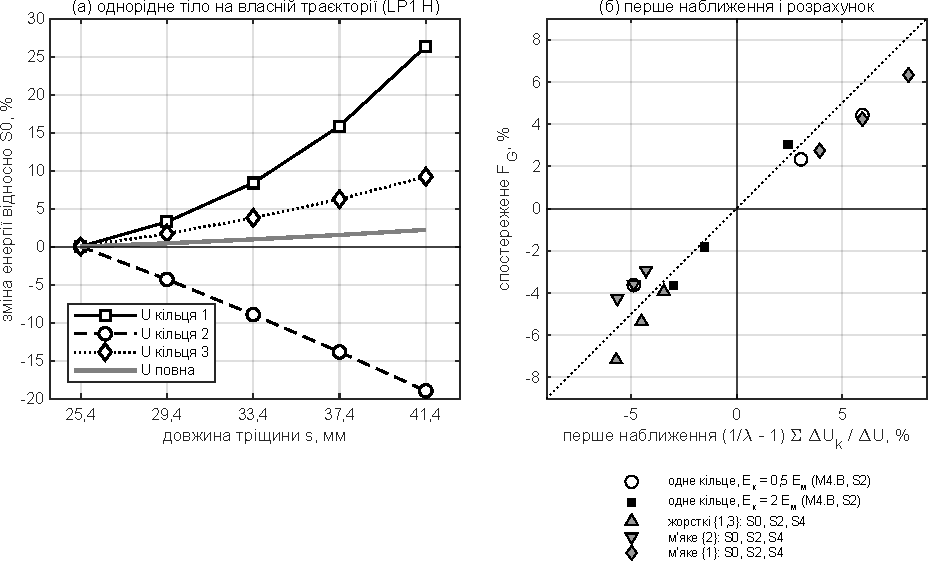
\includegraphics[width=\textwidth]{figures/G1_5_energii_kilets_UA.pdf}
 \caption{Зміна енергії в областях кілець уздовж однорідної траєкторії (а); зіставлення оцінки першого порядку та обчислених енергетичних контрастів (б). Частина архітектурних порівнянь виконана на різних власних траєкторіях.}
 \label{fig:ring-energy-evolution}
\end{figure}

Енергія в області кільця 2 монотонно зменшується на досліджених дискретних станах, тоді як в областях кілець 1 і 3 зростає. Це відповідає і змінам усереднених головних напружень: у кільці 2 модуль меншого головного напруження зменшується приблизно від $4{,}04$ до $3{,}50$ в одиницях $10^{-4}$ МПа, у кільці 1 збільшується розтягальна складова, у кільці 3 --- стискальна. Таким чином, відмінність полягає у характері перерозподілу енергії при рості тріщини, а не просто в наявності стиску.

\subsection{Кількісна перевірка оцінки першого порядку}

Для S2 застосуємо центральну різницю між S1 і S3:
\begin{equation}
 b_k^{\mathrm{FD}}=
 \frac{\mathcal W_k^{\mathrm H}(S3)-\mathcal W_k^{\mathrm H}(S1)}
 {\mathcal W_{\mathrm H}(S3)-\mathcal W_{\mathrm H}(S1)}.
 \label{eq:ring-b-fd}
\end{equation}
Інтервал довжини 8 мм скорочується у відношенні. Отримуємо $b_1=0{,}05959$, $b_2=-0{,}04872$, $b_3=0{,}03050$. Зіставимо $\eta_k b_k$ із результатами прямих розрахунків одиночних кілець.

\begin{table}[htbp]
 \centering
 \caption{Оцінка першого порядку та прямі розрахунки для одиночних кілець на S2, \%}
 \label{tab:ring-first}
 \begin{tabular}{rrrrr}
 \toprule
 & \multicolumn{2}{c}{$\lambda=0{,}5$} & \multicolumn{2}{c}{$\lambda=2$}\\
 \cmidrule(lr){2-3}\cmidrule(lr){4-5}
 Кільце & Оцінка & Розрахунок & Оцінка & Розрахунок\\
 \midrule
 1 & $+5,96$ & $+4,43$ & $-2,98$ & $-3,65$\\
 2 & $-4,87$ & $-3,63$ & $+2,44$ & $+3,04$\\
 3 & $+3,05$ & $+2,33$ & $-1,52$ & $-1,82$\\
 \bottomrule
 \end{tabular}
\end{table}

Знаки збігаються для всіх шести одиночних випадків. Для м'яких кілець оцінка завищує модуль ефекту, для жорстких --- занижує. Зіставлення з другою зовнішньою сіткою дає майже такі самі відношення обчисленого ефекту до оцінки. Додатково за збереженими однорідними станами виконано односторонні різниці на S0 та S4 і центральну на S2 для трьох вибраних архітектур. При S0 геометрія спільна; при S2 і S4 обчислений повний контраст містить також вплив різниці траєкторій. У сумі знаки збіглися в 21 із 21 пов'язаного порівняння (12 одиночних на двох сітках та 9 архітектурних). Це не 21 незалежне статистичне випробування.

Для м'яких архітектур і одиночних кілець відношення розрахунку до оцінки становить приблизно 0,68--0,78, для жорстких --- 1,14--1,26. Відхилення від оцінки сягають 14--32\,\% від її модуля. Це спостережені розбіжності за скінченного контрасту та різницевого наближення похідних; їх не можна ідентифікувати як виміряний член саме другого порядку. Для такого висновку потрібна серія малих контрастів і окрема перевірка похідної форми. Більш того, пізніші прямі перехресні розрахунки S4 не підтвердили наперед задані інтервали оцінки для stiff13 та soft1 (див. наступний розділ). Тому оцінка першого порядку пояснює знакову тенденцію, але не є універсальним кількісним предиктором.

\subsection{Просторова карта чутливості}

Вираз~\eqref{eq:ring-first-G} допускає просторове узагальнення. Для малої зміни матеріальної податливості $\eta(\boldsymbol x)$ в області, яка не перетинає тріщину чи її віртуальний приріст, введемо
\begin{equation}
 \iota(\boldsymbol x)=
 \frac{\partial_s w_{\mathrm H}(\boldsymbol x)}
 {\partial_s\mathcal W_{\mathrm H}},\qquad
 F_G^{(1)}=\int_\Omega\eta(\boldsymbol x)\iota(\boldsymbol x)
 \,\mathrm d\Omega .
 \label{eq:ring-influence}
\end{equation}
Густина $\iota$ має розмірність мм$^{-2}$. Її від'ємне значення означає екранувальну тенденцію при малому пом'якшенні відповідної області, додатне --- тенденцію підсилення. Це поле чутливості, а не густина енергії.

\begin{figure}[htbp]
 \centering
 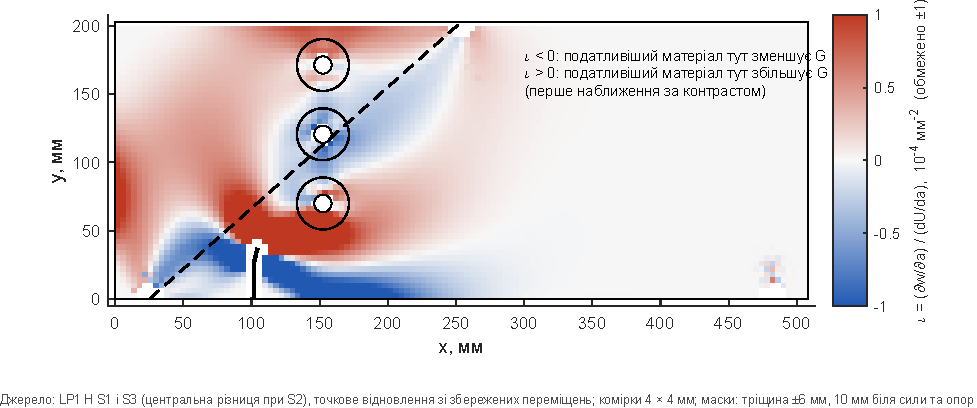
\includegraphics[width=\textwidth]{figures/G1_4_karta_vplyvu_UA.pdf}
 \caption{Різницеве наближення густини чутливості $\iota$ на S2 за однорідними полями S1 та S3. Масковано окіл тріщини й точки закріплення та навантаження; шкалу обмежено $\pm10^{-4}$ мм$^{-2}$.}
 \label{fig:ring-influence}
\end{figure}

Карту отримано точковим відновленням полів S1 та S3 на спільній координатній сітці з кроком 1 мм та усередненням по комірках 4 на 4 мм. Тріщину і зони по 10 мм навколо опор та сили виключено; біля тріщини ширина маски становить 6 мм з кожного боку. Інтегрування карти по кільцях дає приблизно 0,0606, $-0{,}0487$ та 0,0296, що відрізняється від~\eqref{eq:ring-b-fd} не більше ніж приблизно на 3\,\%. Різниця відображає просторове усереднення, маскування і різну дискретизацію станів; карта не є сертифікованою похідною.

Від'ємна область на боці сили охоплює кільце 2. Уздовж вертикальної лінії центрів кілець від'ємна смуга займає приблизно $82<y<158$ мм; кільце 2 повністю лежить у цьому інтервалі за висотою, кільця 1 і 3 зачеплені краями. Це пояснює знаки інтегральних чутливостей. На боці опори картина інша, а поблизу тріщини істотним є її власне ближнє поле. Необхідно уникати тлумачення всієї прямої опора--сила як єдиного силового стрижня.

\section{Вибір архітектур і межі фізичного пояснення}
\label{sec:ring-summary}

Проведене дослідження дозволило встановити, що розташування однакових за площею неоднорідностей змінює як знак, так і величину прямого енергетичного ефекту. Для пояснення протилежної ролі кільця 2 найбільш змістовним є не знак напруження, а енергетична чутливість до зміни геометрії тріщини. Її різницеве наближення відтворює знаки ефектів і дає правильний порядок величини. При цьому гіпотезу про розвантаження діагональної області передачі стискальних напружень підтверджено лише частково. Для виділення саме цього механізму необхідні контрольовані зміни положення сили, опор або кільця при збереженні інших параметрів. Такого розрахункового експерименту не виконано.

Для подальшої побудови власних траєкторій вибрано три архітектури: stiff13 --- жорсткі кільця 1 і 3 з найбільшим обчисленим екрануванням у серії S2; soft2 --- м'яке кільце 2 з від'ємним енергетичним ефектом і відносно малим напрямним ефектом; soft1 --- м'яке кільце 1 з підсиленням рушійної сили й істотним напрямним ефектом протилежного знака. Однорідна конфігурація H є опорною. Вибір забезпечує різні поєднання енергетичного та напрямного ефектів, а не три варіанти одного й того самого механізму.

Результат для soft2 на фіксованій S2 розрізняється за обома критеріями саме в цій серії. Це не гарантує консервативного розрізнення повного ефекту на наступних власних геометріях. Після незалежного розвитку тріщини прямий ефект матеріалу вже не збігається з повним ефектом, оскільки матеріал змінює також геометрію. Для розмежування цих двох впливів необхідні перехресні розрахунки. Їм присвячено наступний розділ.

\chapter{Взаємодія матеріальних характеристик і геометрії тріщини}
\label{ch:feedback}

У розділах~\ref{ch:fixed-crack} і~\ref{ch:ring-placement} матеріальний ефект досліджено за заданих геометрій. Така постановка дозволяє встановити прямий вплив неоднорідності, але не враховує того, що в процесі розвитку тріщини матеріал визначає її напрямок, а нова геометрія змінює наступний пружний розв'язок. У цьому розділі розмежуємо ці впливи. Задача полягає не у визначенні незалежних фізичних причин, а в контрольованому порівнянні пружних розв'язків для матеріалу та геометрії, які можна задавати окремо, хоча під час побудови траєкторії вони пов'язані.

\section{Зворотний зв'язок і факторний план}
\label{sec:feedback-design}

Позначимо через $\Gamma_{X,n}$ ламану тріщину в матеріалі $X$ після $n$ умовних приростів, через $\varphi_{X,n}$ кут дотичної її останнього відрізка, а через $\theta_{X,n}$ локальний кут МКН. На спільній початковій геометрії $\Gamma_{X,0}=\Gamma_{\mathrm H,0}$ матеріал уже змінює КІН. Наступна геометрія визначається співвідношенням~\eqref{eq:problem-step}. У позначеннях операторів цей зворотний зв'язок можна подати як
\begin{equation}
 (X,\Gamma_{X,n})\longmapsto
 (\KI,\KII)_{X,n}\longmapsto\theta_{X,n}
 \longmapsto \Gamma_{X,n+1}.
 \label{eq:feedback-map}
\end{equation}
Порівнюємо стани за однакової довжини $s$, а не за однакових координат вершини. Умовні прирости однакові за довжиною; ні час, ні критичне навантаження не визначаються.

Для довільної архітектури $X$ і величини $Q$ (наприклад $G$ або $\KI$) утворимо чотири конфігурації:
\begin{equation}
 \begin{array}{c|cc}
 &\Gamma_{\mathrm H}&\Gamma_X\\ \hline
 \mathrm H & Q_{\mathrm{HH}} & Q_{\mathrm{HX}}\\
 X & Q_{\mathrm{XH}} & Q_{\mathrm{XX}}
 \end{array}
 \label{eq:feedback-factorial}
\end{equation}
Перший індекс означає матеріал, другий --- геометрію. Діагональні розв'язки належать власним траєкторіям, позадіагональні --- контрольним задачам. Зокрема, $\Gamma_X$ в однорідному матеріалі є заданою геометрією, а не траєкторією, яку однорідне тіло самостійно вибрало за критерієм МКН.

Якщо $Q_{\mathrm{HH}}>0$, введемо нормований розклад
\begin{equation}
 \begin{aligned}
 F_{\mathrm m}&=(Q_{\mathrm{XH}}-Q_{\mathrm{HH}})/Q_{\mathrm{HH}},\\
 F_{\mathrm p}&=(Q_{\mathrm{HX}}-Q_{\mathrm{HH}})/Q_{\mathrm{HH}},\\
 F_{\mathrm i}&=(Q_{\mathrm{XX}}-Q_{\mathrm{XH}}-
                  Q_{\mathrm{HX}}+Q_{\mathrm{HH}})/Q_{\mathrm{HH}},\\
 F_{\mathrm{tot}}&=F_{\mathrm m}+F_{\mathrm p}+F_{\mathrm i}.
 \end{aligned}
 \label{eq:feedback-additive}
\end{equation}
Тут $F_{\mathrm m}$ --- прямий матеріальний внесок на однорідній геометрії; $F_{\mathrm p}$ --- внесок геометрії в однорідному матеріалі; $F_{\mathrm i}$ --- перехресна різниця (зміна матеріального внеску внаслідок заміни геометрії). Останній член не слід ототожнювати з міжкільцевими взаємодіями розділу~\ref{ch:ring-placement}. Для локального кута використовуємо абсолютні різниці в градусах, тобто ті самі чисельники без ділення. Для другого КІН нормуємо всі чотири значення на одну опорну норму $K_0=[K_{\mathrm I,HH}^2+K_{\mathrm{II},HH}^2]^{1/2}$, а потім беремо їхні різниці. Таке нормування не вироджується поблизу чистої моди I.

Часто є лише три з чотирьох розв'язків. У такому разі можна встановити лише послідовний внесок заміни геометрії в матеріалі $X$:
\begin{equation}
 F_{\mathrm p}+F_{\mathrm i}
 =\frac{Q_{\mathrm{XX}}-Q_{\mathrm{XH}}}{Q_{\mathrm{HH}}}.
 \label{eq:feedback-sequential}
\end{equation}
Якщо всі $Q$ додатні, той самий облік можна записати через відношення
\begin{equation}
 R_{\mathrm{dir}}=\frac{Q_{\mathrm{XH}}}{Q_{\mathrm{HH}}},
 \quad R_{\mathrm{seq}}=\frac{Q_{\mathrm{XX}}}{Q_{\mathrm{XH}}},
 \quad R_{\mathrm{tot}}=R_{\mathrm{dir}}R_{\mathrm{seq}}.
 \label{eq:feedback-ratio}
\end{equation}
У цьому записі $R_{\mathrm{seq}}$ не є чистим геометричним відношенням $Q_{\mathrm{HX}}/Q_{\mathrm{HH}}$. Це важлива відмінність ранніх серій від повного факторного плану.

\section{Перші власні траєкторії: одночасна активація трьох кілець}
\label{sec:feedback-m3}

Після розрахунків із замороженою тріщиною вперше виконано незалежне продовження однорідної, трьох м'яких та трьох жорстких кілець на два прирости по 4 мм. Конфігурації цієї ранньої серії M3 не збігаються з soft1, soft2 і stiff13. Результати дають змогу визначити послідовний, але не чистий геометричний внесок.

\begin{table}[htbp]
 \centering
 \caption{Послідовний розклад $G$ для трьох однаково активованих кілець (вихідне сімейство сіток). Останній стовпець --- відсоткові пункти.}
 \label{tab:feedback-m3}
 \begin{tabular}{lrrrr}
 \toprule
 Конфігурація / стан & $R_{\mathrm{dir}}$ & $R_{\mathrm{seq}}$ & $R_{\mathrm{tot}}$ & $100(F_{\mathrm p}+F_{\mathrm i})$\\
 \midrule
М'які / S1 & $1,006199$ & $0,999511$ & $1,005706$ & $-0,0492$ \\
М'які / S2 & $1,021813$ & $0,998826$ & $1,020614$ & $-0,1199$ \\
Жорсткі / S1 & $0,981870$ & $1,000396$ & $0,982259$ & $+0,0389$ \\
Жорсткі / S2 & $0,970687$ & $1,000813$ & $0,971476$ & $+0,0789$ \\

 \bottomrule
 \end{tabular}
\end{table}

На S0 геометрія спільна, тому $R_{\mathrm{seq}}=1$. Після двох приростів для м'яких кілець заміна геометрії в тому самому матеріалі послаблює підсилення, а для жорстких послаблює екранування. Обидва ефекти малі порівняно з прямим внеском. Знак енергетичного контрасту м'яких кілець, розглянутий у розділі~\ref{ch:fixed-crack}, змінюється і на власній траєкторії. Усі ненульові відношення розрізняються за первинним критерієм M3, але не за консервативним.

\begin{figure}[htbp]
 \centering
 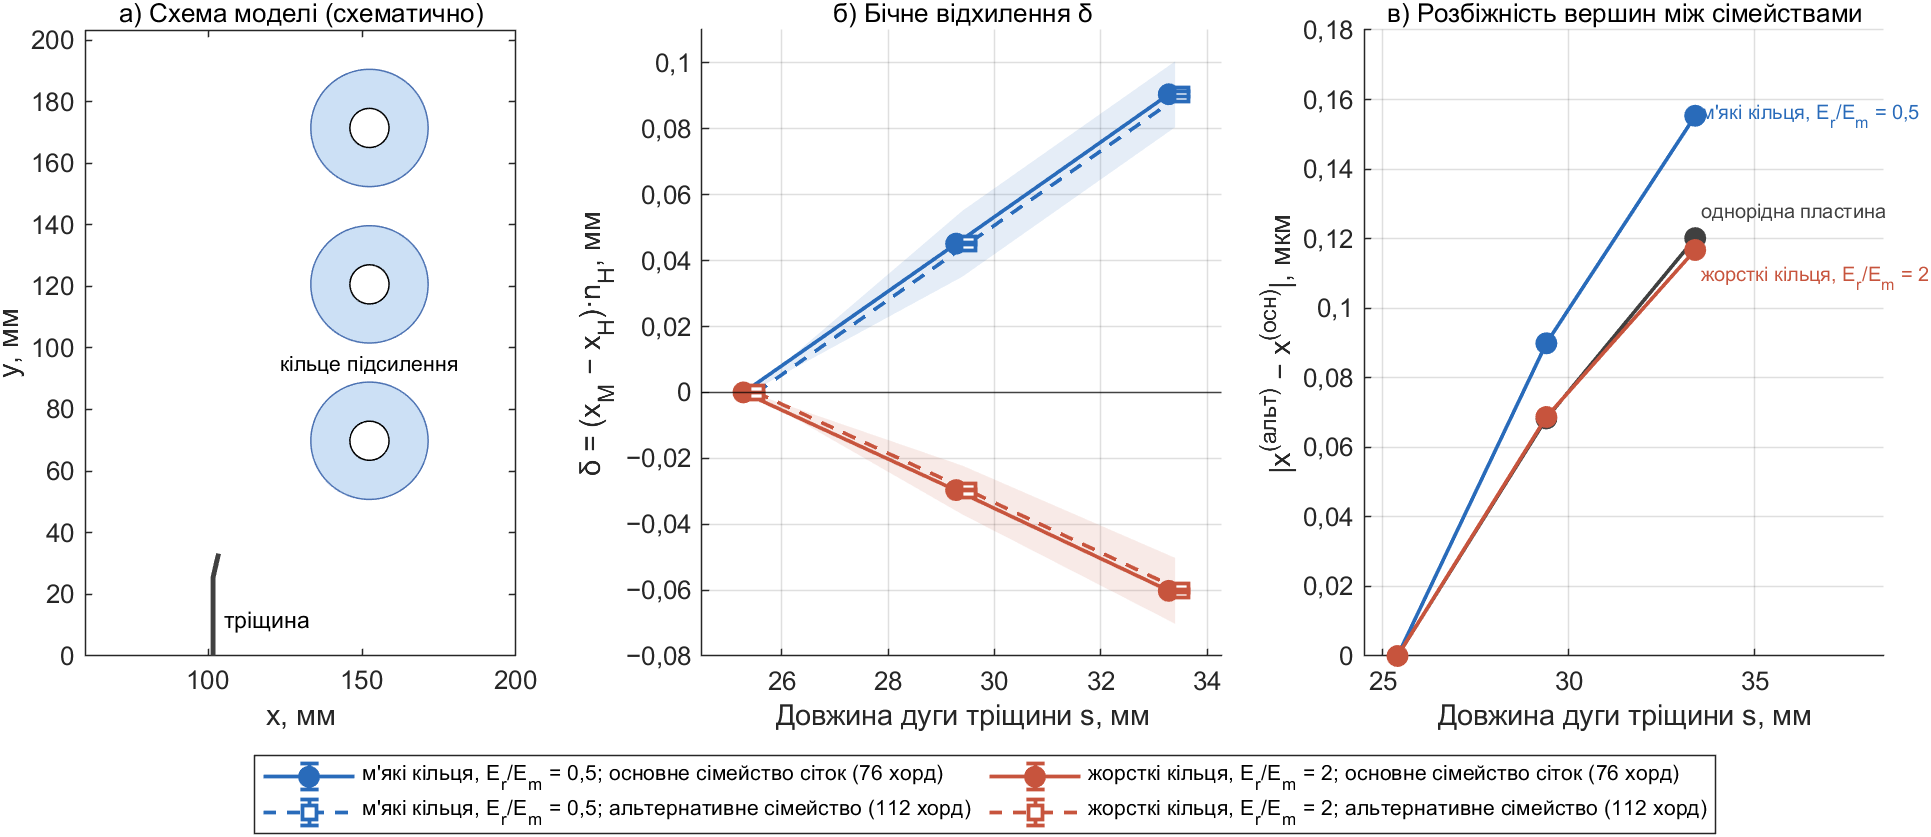
\includegraphics[width=\textwidth]{figures/m4a_fig1_paths.png}
 \caption{Порівняння двокрокових траєкторій із трьома активними кільцями на двох зовнішніх сімействах сіток. Бічні відхилення та міжсіткову розбіжність наведено окремо.}
 \label{fig:feedback-m4a-paths}
\end{figure}

\begin{figure}[htbp]
 \centering
 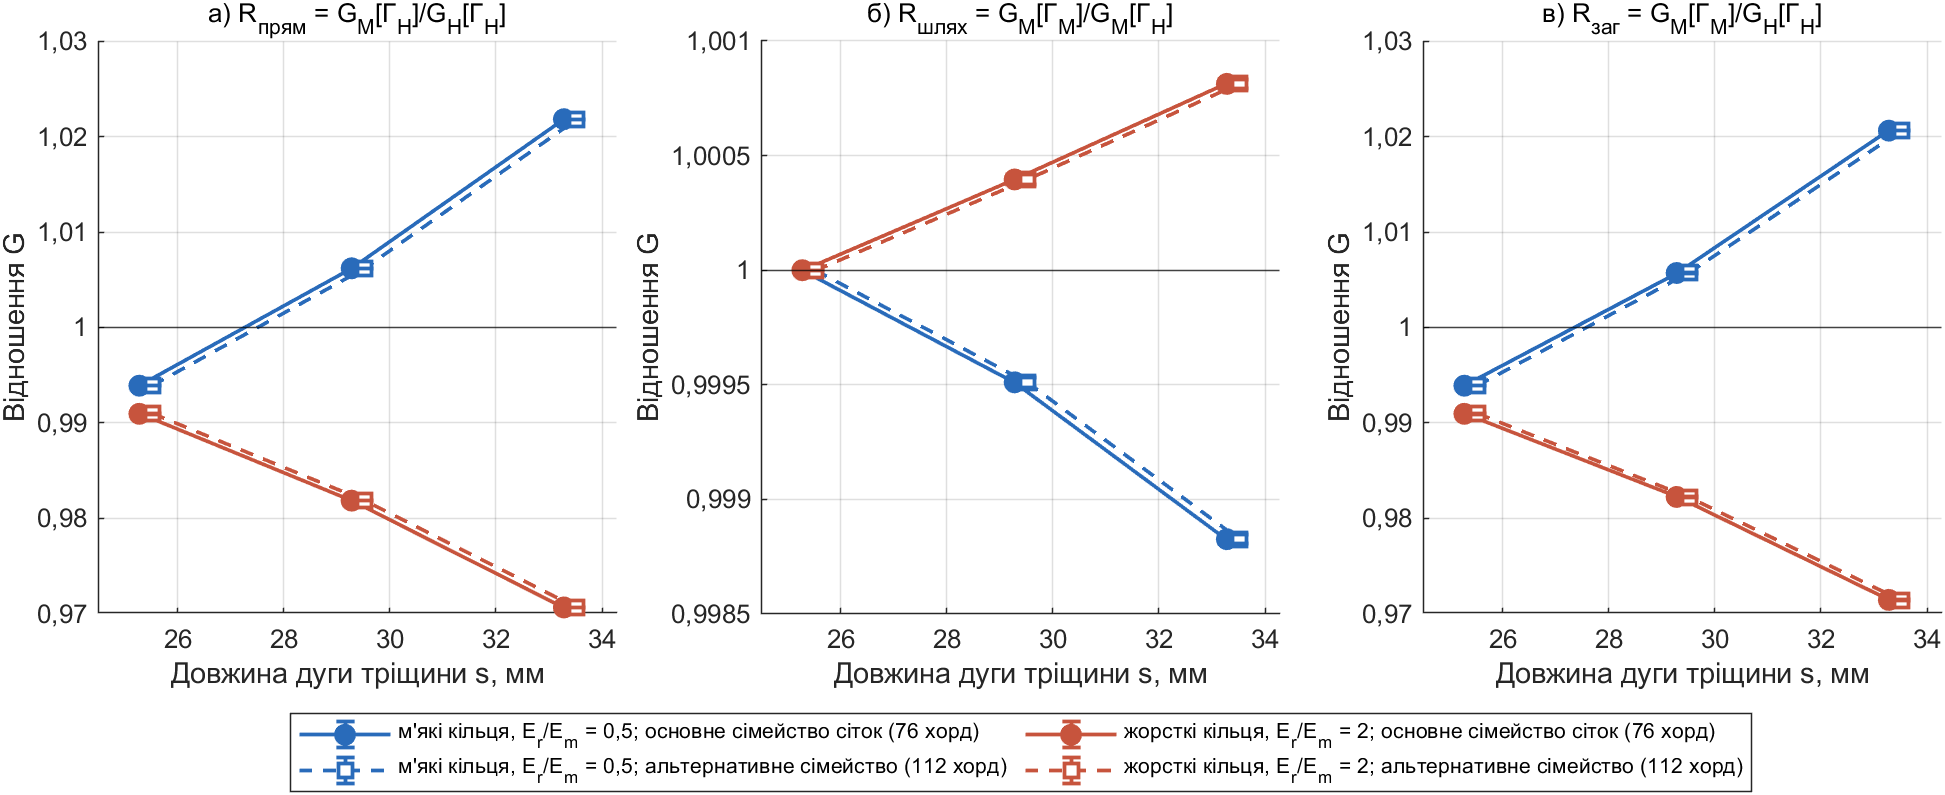
\includegraphics[width=\textwidth]{figures/m4a_fig2_ratios.png}
 \caption{Відношення прямого, послідовного та повного ефектів для двох сімейств сіток. Смуги відповідають первинному індикатору, а не гарантованій похибці.}
 \label{fig:feedback-m4a-ratios}
\end{figure}

Для цих коротких траєкторій у M4.A незалежно повторено весь двокроковий розрахунок на альтернативному сімействі зовнішніх сіток із 112 хордами замість 76, зберігаючи привершинне ядро. На S2 для м'яких кілець $R_{\mathrm{seq}}$ становить 0,998826 на обох сімействах із точністю до шести знаків, для жорстких --- 1,000813. Бічне зміщення відносно однорідного шляху становить відповідно $+0{,}09050$ та $-0{,}06022$ мм; заміна сімейства змінює його на $3{,}5\cdot10^{-5}$ та $-3{,}4\cdot10^{-6}$ мм. Таким чином, підтверджено стійкість саме двокрокового спостереження до однієї конкретної зміни зовнішньої дискретизації. Дослідження не охоплює локального подрібнення ядра, зменшення приросту $\Delta a$ чи довших траєкторій.

\section{Прямий та повний ефекти вибраних архітектур на S0--S4}
\label{sec:feedback-existing}

Для архітектур, вибраних у розділі~\ref{ch:ring-placement}, незалежно побудовано чотири власні траєкторії до S4. На S0 усі 23 поля масивів сіток збігаються; різні SHA сирих MAT-файлів пояснюються відмінністю метаданих. Отже, на S0 прямий та повний ефекти збігаються на рівні дискретного розв'язку. На S2 доступні прямі розрахунки M4.B, а також власні LP1/A0. Однорідні опорні значення $G$ цих історичних серій відрізняються приблизно на $8\cdot10^{-8}$ відносно одне одного; тому зіставлення їхніх нормованих контрастів є наближеним міжсерійним порівнянням, а не точною тотожністю чотирьох записів однієї кампанії.

\begin{table}[htbp]
 \centering
 \caption{Прямі та повні контрасти $G$ вибраних архітектур, \%. Стовпець залишку --- відсоткові пункти.}
 \label{tab:feedback-s2}
 \begin{tabular}{lrrrr}
 \toprule
 & S0 & \multicolumn{3}{c}{S2}\\
 \cmidrule(lr){3-5}
 Архітектура & $F_{\mathrm{tot}}=F_{\mathrm m}$ & $F_{\mathrm m}$ & $F_{\mathrm{tot}}$ & $F_{\mathrm p}+F_{\mathrm i}$\\
 \midrule
stiff13 & $-3,9312$ & $-5,4780$ & $-5,3478$ & $+0,1301$ \\
soft2 & $-4,2590$ & $-3,6278$ & $-3,5768$ & $+0,0510$ \\
soft1 & $+2,7458$ & $+4,4298$ & $+4,2395$ & $-0,1903$ \\

 \bottomrule
 \end{tabular}
\end{table}

Для всіх трьох архітектур на S2 залишок протилежний прямому ефекту. Відсутні розрахунки $\mathrm H$ на $\Gamma_X$, тому окремо встановити знак $F_{\mathrm p}$ та $F_{\mathrm i}$ на S2 неможливо. Перші спостереження мотивували наступний розрахунковий експеримент на S4.

\begin{figure}[htbp]
 \centering
 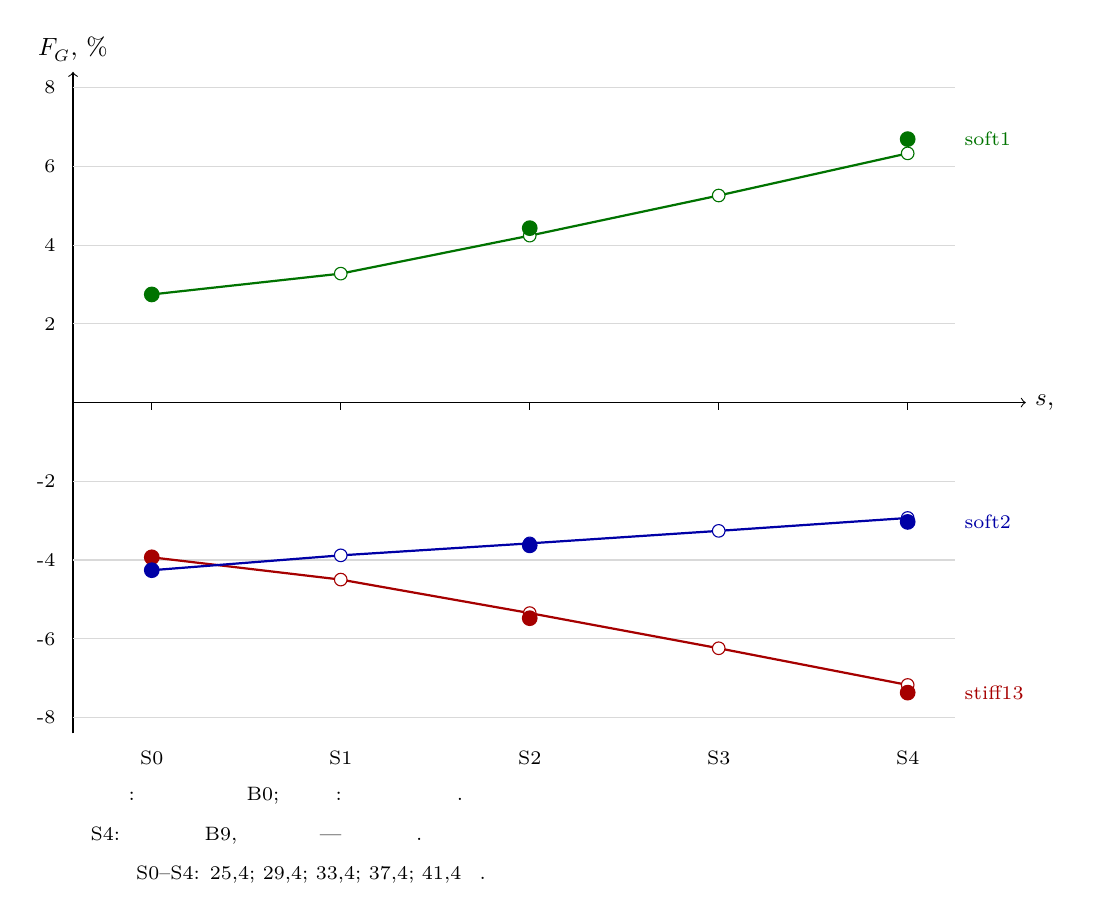
\begin{tikzpicture}[x=1mm,y=1mm,font=\small]
 \draw[->] (0,0)--(121,0) node[right] {$s$, мм};
 \draw[->] (0,-42)--(0,42) node[above] {$F_G$, \%};
 \foreach \v in {-8,-6,-4,-2,2,4,6,8}{
  \draw[black!15] (0,5*\v)--(112,5*\v);
  \node[anchor=east,font=\scriptsize] at (-1,5*\v) {\v};
 }
 \foreach \i/\s in {0/25,1/29,2/33,3/37,4/41}{
  \draw (10+24*\i,0)--(10+24*\i,-1);
  \node[anchor=north,font=\scriptsize] at (10+24*\i,-43) {S\i};
 }
\draw[red!65!black,line width=.8pt] (10,-19.65607)--(34,-22.48607)--(58,-26.73923)--(82,-31.20558)--(106,-35.86585);
\draw[red!65!black,fill=white] (10,-19.65607) circle[radius=.8mm];
\draw[red!65!black,fill=white] (34,-22.48607) circle[radius=.8mm];
\draw[red!65!black,fill=white] (58,-26.73923) circle[radius=.8mm];
\draw[red!65!black,fill=white] (82,-31.20558) circle[radius=.8mm];
\draw[red!65!black,fill=white] (106,-35.86585) circle[radius=.8mm];
\fill[red!65!black] (10,-19.65607) circle[radius=1mm];
\fill[red!65!black] (58,-27.38978) circle[radius=1mm];
\fill[red!65!black] (106,-36.84178) circle[radius=1mm];
\node[anchor=west,font=\scriptsize,text=red!65!black] at (112,-36.84178) {stiff13};
\draw[blue!65!black,line width=.8pt] (10,-21.29476)--(34,-19.40687)--(58,-17.88408)--(82,-16.29774)--(106,-14.65908);
\draw[blue!65!black,fill=white] (10,-21.29476) circle[radius=.8mm];
\draw[blue!65!black,fill=white] (34,-19.40687) circle[radius=.8mm];
\draw[blue!65!black,fill=white] (58,-17.88408) circle[radius=.8mm];
\draw[blue!65!black,fill=white] (82,-16.29774) circle[radius=.8mm];
\draw[blue!65!black,fill=white] (106,-14.65908) circle[radius=.8mm];
\fill[blue!65!black] (10,-21.29476) circle[radius=1mm];
\fill[blue!65!black] (58,-18.13920) circle[radius=1mm];
\fill[blue!65!black] (106,-15.15980) circle[radius=1mm];
\node[anchor=west,font=\scriptsize,text=blue!65!black] at (112,-15.15980) {soft2};
\draw[green!45!black,line width=.8pt] (10,13.72911)--(34,16.37179)--(58,21.19736)--(82,26.29237)--(106,31.64468);
\draw[green!45!black,fill=white] (10,13.72911) circle[radius=.8mm];
\draw[green!45!black,fill=white] (34,16.37179) circle[radius=.8mm];
\draw[green!45!black,fill=white] (58,21.19736) circle[radius=.8mm];
\draw[green!45!black,fill=white] (82,26.29237) circle[radius=.8mm];
\draw[green!45!black,fill=white] (106,31.64468) circle[radius=.8mm];
\fill[green!45!black] (10,13.72911) circle[radius=1mm];
\fill[green!45!black] (58,22.14903) circle[radius=1mm];
\fill[green!45!black] (106,33.45580) circle[radius=1mm];
\node[anchor=west,font=\scriptsize,text=green!45!black] at (112,33.45580) {soft1};
 \node[anchor=west,font=\scriptsize] at (1,-50) {Порожні: власна траєкторія B0; заповнені: фіксована геометрія.};
 \node[anchor=west,font=\scriptsize] at (1,-55) {S4: прямий ефект B9, решта станів --- базові сітки.};
 \node[anchor=west,font=\scriptsize] at (1,-60) {Довжини S0--S4: 25,4; 29,4; 33,4; 37,4; 41,4 мм.};
\end{tikzpicture}

 \caption{Повні енергетичні контрасти власних траєкторій та прямі матеріальні контрасти у вибраних станах. Значення S4 для прямого ефекту отримано в кампанії X6 на B9; лінії з'єднують повні контрасти на базовій дискретизації B0, не є інтерполяцією прямого ефекту.}
 \label{fig:feedback-direct-total}
\end{figure}

\section{Шість перехресних розрахунків S4}
\label{sec:feedback-x6}

Для повного факторного плану на $s=41{,}4$ мм використано чотири збережені геометрії та відповідні сітки локального рівня B9 з дослідження A1. Діагональні розв'язки не перераховували. Для кожної архітектури виконано дві задачі: матеріал $X$ на сітці $\Gamma_{\mathrm H}$ та однорідний матеріал на сітці $\Gamma_X$. Усередині кожної геометрії сітка не змінювалася. Усі шість задач пройшли 16 критеріїв визначення КІН, окремі перевірки фаз та відповідності матеріальної конфігурації. Повторне читання записів підтвердило їхню цілісність без нових розв'язків. Наукове приймання стосується саме цих шести задач, а не інших станів траєкторії.

\begin{table}[htbp]
 \centering
 \caption{Чотири енергетичні значення факторного плану S4 на B9, в одиницях $10^{-8}$ Н/мм при силі 1 Н.}
 \label{tab:feedback-cross}
 \begin{tabular}{lrrrr}
 \toprule
 Архітектура & $G_{\mathrm{HH}}$ & $G_{\mathrm{XH}}$ & $G_{\mathrm{HX}}$ & $G_{\mathrm{XX}}$\\
 \midrule
stiff13 & $1,539127$ & $1,425719$ & $1,542243$ & $1,428716$ \\
soft2 & $1,539127$ & $1,492461$ & $1,540581$ & $1,494004$ \\
soft1 & $1,539127$ & $1,642112$ & $1,533379$ & $1,636545$ \\

 \bottomrule
 \end{tabular}
\end{table}

\begin{table}[htbp]
 \centering
 \caption{Розклад енергетичного контрасту на S4, \%. Останній стовпець --- частка прямого ефекту, компенсована зміною геометрії: $\rho_{\mathrm c}=-100(F_{\mathrm p}+F_{\mathrm i})/F_{\mathrm m}$.}
 \label{tab:feedback-G}
 \begin{tabular}{lrrrrr}
 \toprule
 Архітектура & $F_{\mathrm m}$ & $F_{\mathrm p}$ & $F_{\mathrm i}$ & $F_{\mathrm{tot}}$ & $\rho_{\mathrm c}$\\
 \midrule
stiff13 & $-7,3684$ & $+0,2024$ & $-0,0077$ & $-7,1736$ & $2,64$ \\
soft2 & $-3,0320$ & $+0,0945$ & $+0,0058$ & $-2,9317$ & $3,31$ \\
soft1 & $+6,6912$ & $-0,3735$ & $+0,0117$ & $+6,3294$ & $5,41$ \\

 \bottomrule
 \end{tabular}
\end{table}

\begin{figure}[htbp]
 \centering
 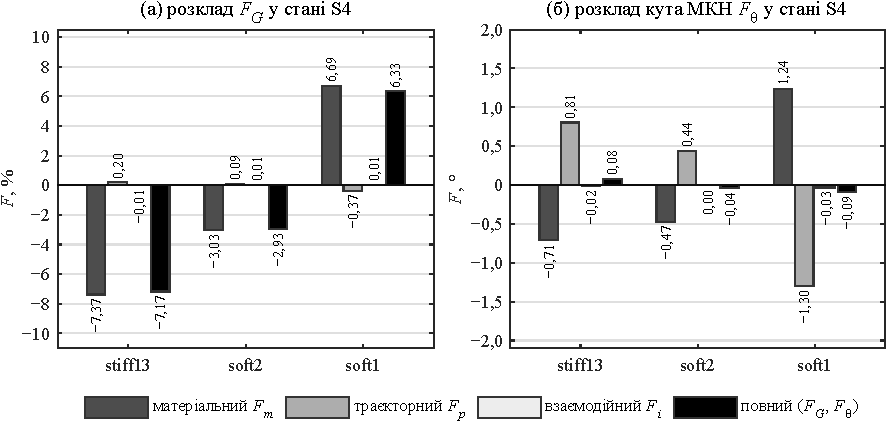
\includegraphics[width=\textwidth]{figures/F07_1_rozklad_S4.pdf}
 \caption{Розклад енергетичного контрасту та зміни локального кута МКН на S4 (B9). Шкали двох панелей різні; усі внески відраховано від стану H на однорідній геометрії.}
 \label{fig:feedback-x6}
\end{figure}

На S4 матеріальний внесок становить 102,7; 103,4 та 105,7\,\% від модуля відповідного повного енергетичного контрасту. Внесок геометрії має протилежний знак у всіх трьох архітектурах. Взаємодія набагато менша за два основні внески, її знак не є однаковим. Заміна геометрії в матеріалі архітектури компенсує приблизно 2,6--5,4\,\% прямого ефекту. Застосування такого самого розкладу до $J$ дає близькі результати (найбільша абсолютна відмінність окремого члена розкладу від розкладу $G$ менша за $2\cdot10^{-6}$ у безрозмірній шкалі).

Перехресні внески обчислено на одному рівні B9. Раніше спостережена зміна енергетичного контрасту при заміні сімейства на S2 ($U_m=3{,}1\cdot10^{-5}$) є лише орієнтиром. Навіть якщо $|F_{\mathrm i}|>2U_m$, з цього не випливає розрізнення взаємодії на S4. Для soft2 $|F_{\mathrm i}|$ менше $2U_m$. Локальне подрібнення діагональних розв'язків A1 не визначає похибки перехресних задач. Консервативну класифікацію soft2 для повного ефекту на власній траєкторії залишено без змін.

\subsection{Залежність від опорного стану та шкали}

Розклад~\eqref{eq:feedback-additive} точний, але залежить від опорної конфігурації. Якщо визначати матеріальний внесок на геометрії $\Gamma_X$ (за того самого нормування на $Q_{\mathrm{HH}}$), він становитиме $F_{\mathrm m}+F_{\mathrm i}$. Симетричний спосіб розподілу взаємодії між матеріалом і геометрією дає
\begin{equation}
 \Phi_{\mathrm m}=F_{\mathrm m}+\tfrac12 F_{\mathrm i},
 \quad \Phi_{\mathrm p}=F_{\mathrm p}+\tfrac12 F_{\mathrm i}.
 \label{eq:feedback-shapley}
\end{equation}
Їхня сума дорівнює повному ефекту. Для додатних $Q$ можливий також мультиплікативний облік:
\begin{equation}
 R_{\mathrm m}=\frac{Q_{\mathrm{XH}}}{Q_{\mathrm{HH}}},
 \quad R_{\mathrm p}=\frac{Q_{\mathrm{HX}}}{Q_{\mathrm{HH}}},
 \quad R_{\mathrm i}=\frac{Q_{\mathrm{XX}}Q_{\mathrm{HH}}}
 {Q_{\mathrm{XH}}Q_{\mathrm{HX}}},
 \quad R_{\mathrm{tot}}=R_{\mathrm m}R_{\mathrm p}R_{\mathrm i}.
 \label{eq:feedback-mult}
\end{equation}
Тут $R_{\mathrm i}$ не дорівнює $1+F_{\mathrm i}$, оскільки множення основних відношень уже містить перехресний добуток. Для енергетичних даних S4 зміна матеріального внеску при переході від $\Gamma_{\mathrm H}$ до $\Gamma_X$ не перевищує 0,012 відсоткового пункта. Тому висновки про домінування прямого внеску та його часткову компенсацію стійкі до цих конкретних способів обліку. Проте жоден не є єдиним фізичним поділом: геометрія $\Gamma_X$ сама виникла внаслідок дії матеріалу на попередніх кроках.

\section{Напрямні ефекти та геометрична пам'ять}
\label{sec:feedback-direction}

Для КІН моди I отримуємо подібний до $G$ характер розкладу. Для КІН моди II та локального кута МКН, навпаки, два основні внески майже компенсуються (табл.~\ref{tab:feedback-angle}). Тут усі $K_{\mathrm{II}}$ нормовано на одну й ту саму опорну норму $K_0$; не йдеться про відношення до власної норми КІН кожної задачі.

\begin{table}[htbp]
 \centering
 \caption{Розклади зміни КІН і локального кута МКН на S4. Нормування зазначено в першому стовпці.}
 \label{tab:feedback-angle}
 \small
 \begin{tabular}{lrrrr}
 \toprule
 Архітектура / величина & Матеріал & Геометрія & Взаємодія & Разом\\
 \midrule
stiff13 / $K_{\mathrm I}$, \% & $-3,7650$ & $+0,1087$ & $+0,0037$ & $-3,6526$ \\
stiff13 / $K_{\mathrm{II}}/K_0$ & $+0,005450$ & $-0,007028$ & $+0,000404$ & $-0,001175$ \\
stiff13 / $\theta$, град & $-0,7113$ & $+0,8057$ & $-0,0166$ & $+0,0778$ \\
soft2 / $K_{\mathrm I}$, \% & $-1,5343$ & $+0,0519$ & $+0,0051$ & $-1,4772$ \\
soft2 / $K_{\mathrm{II}}/K_0$ & $+0,003839$ & $-0,003827$ & $+0,000084$ & $+0,000097$ \\
soft2 / $\theta$, град & $-0,4714$ & $+0,4387$ & $-0,0030$ & $-0,0357$ \\
soft1 / $K_{\mathrm I}$, \% & $+3,3013$ & $-0,2094$ & $+0,0232$ & $+3,1150$ \\
soft1 / $K_{\mathrm{II}}/K_0$ & $-0,010695$ & $+0,011286$ & $+0,000652$ & $+0,001243$ \\
soft1 / $\theta$, град & $+1,2379$ & $-1,2959$ & $-0,0308$ & $-0,0888$ \\

 \bottomrule
 \end{tabular}
\end{table}

Наприклад, для soft1 матеріал на $\Gamma_{\mathrm H}$ збільшив би кут МКН на $1{,}238^\circ$, проте заміна геометрії в однорідному матеріалі зменшує його на $1{,}296^\circ$. З урахуванням взаємодії повна різниця локального кута дорівнює лише $-0{,}089^\circ$. Така компенсація не означає, що координати вершини або напрямок уже утвореної ламаної збігаються.

Дійсно, якщо $\Delta\varphi_n=\varphi_{X,n}-\varphi_{\mathrm H,n}$, а $\Delta\theta_n=\theta_{X,n}-\theta_{\mathrm H,n}$, то
\begin{equation}
 \Delta\varphi_{n+1}=\Delta\varphi_n+\Delta\theta_n,\qquad
 \Delta\varphi_n=\sum_{j=0}^{n-1}\Delta\theta_j.
 \label{eq:feedback-heading}
\end{equation}
Кут $\theta_n$ є прогнозом для наступного приросту, тому не входить до суми для вже утвореного останнього відрізка $n$. Звідси точна геометрична різниця координат
\begin{equation}
 \boldsymbol x_{X,n}-\boldsymbol x_{\mathrm H,n}
 =\Delta a\sum_{k=1}^{n}
 [\boldsymbol\tau(\varphi_{X,k})-\boldsymbol\tau(\varphi_{\mathrm H,k})].
 \label{eq:feedback-tip-sum}
\end{equation}
Проєктуючи на нормаль $\boldsymbol n_{\mathrm H,n}$ та лінеаризуючи за малими різницями кутів у радіанах, отримуємо
\begin{equation}
 d_n=\Delta a\sum_{k=1}^{n}
 \Delta\varphi_k\cos(\varphi_{\mathrm H,k}-\varphi_{\mathrm H,n})
 +O\!\left(\Delta a\sum_{k=1}^{n}|\Delta\varphi_k|^2\right).
 \label{eq:feedback-lateral}
\end{equation}
Таким чином, навіть якщо $\Delta\theta_n$ стає малим, попередні різниці кутів залишаються в $\Delta\varphi_k$ та накопиченому зміщенні $d_n$. Для майже паралельних коротких шляхів і приблизно сталої різниці напрямків після першого приросту маємо грубу оцінку $d_n\simeq n\Delta a\sin(\Delta\theta_0)$. Це не твердження про те, що матеріал діє лише на першому кроці.

\begin{figure}[htbp]
 \centering
 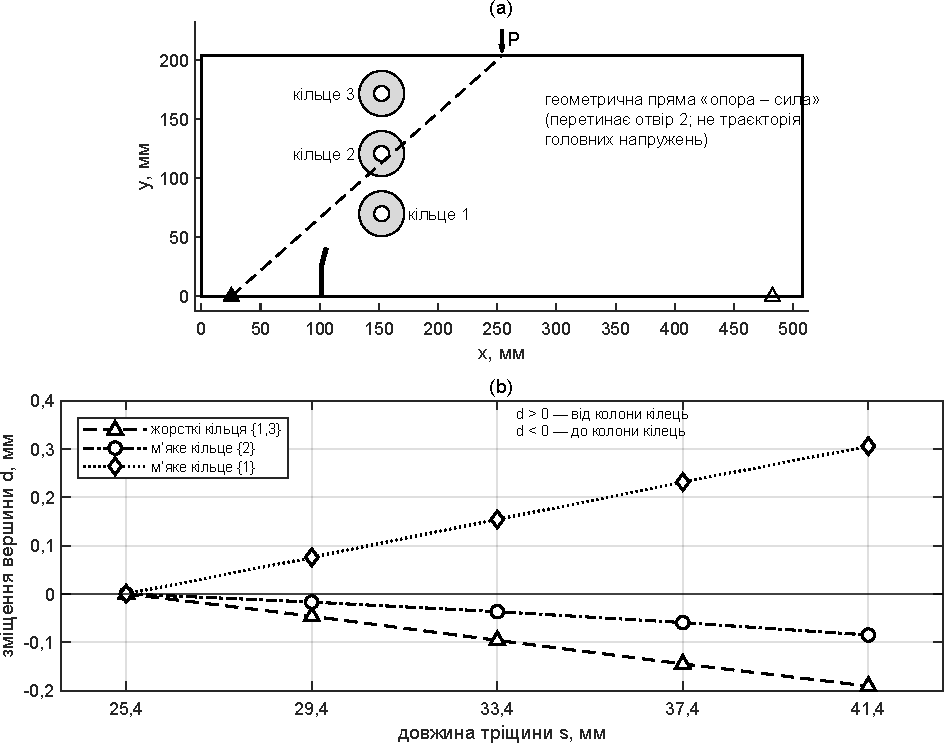
\includegraphics[width=\textwidth]{figures/M5_1_geometriia_UA.pdf}
 \caption{Однорідна траєкторія до S4 і бічні зміщення вибраних архітектур. Пряма опора--сила є геометричним орієнтиром.}
 \label{fig:feedback-offset}
\end{figure}

\begin{table}[htbp]
 \centering
 \caption{Різниці кутів і бічні зміщення на власних траєкторіях S4 (B0). Останній стовпець --- відношення грубої оцінки першого зламу до фактичного зміщення $\rho_1=16\sin\Delta\theta_0/d_4$.}
 \label{tab:feedback-heading}
 \begin{tabular}{lrrrrr}
 \toprule
 & $\Delta\theta_0$, град & $\Delta\varphi_4$, град & $\Delta\theta_4$, град & $d_4$, мм & $\rho_1$\\
 \midrule
stiff13 & $-0,6627$ & $-0,6611$ & $+0,0778$ & $-0,1909$ & $0,969$ \\
soft2 & $-0,2433$ & $-0,3669$ & $-0,0356$ & $-0,0852$ & $0,798$ \\
soft1 & $+1,0842$ & $+1,0682$ & $-0,0888$ & $+0,3057$ & $0,990$ \\

 \bottomrule
 \end{tabular}
\end{table}

Незалежне відновлення координат за~\eqref{eq:feedback-tip-sum} для 12 пар станів S1--S4 дає максимальну розбіжність менше $10^{-12}$ мм, а накопичених кутів за~\eqref{eq:feedback-heading} --- менше $10^{-12}$ градуса. Лінеаризація~\eqref{eq:feedback-lateral} відтворює бічне зміщення з максимальною абсолютною розбіжністю менше $10^{-3}$ мм у цих станах. Ці перевірки стосуються геометричної рекурсії, а не точності прогнозування фізичної траєкторії.

На S4 наближена оцінка на основі першого приросту становить 80--99\,\% фактичного бічного зміщення. Цей збіг підтверджує її придатність як геометричної оцінки для коротких шляхів, але не встановлює причинної частки першого зламу: для цього потрібні контрольні траєкторії із заданою зміною лише одного кроку. Кутова компенсація в факторному плані S4 сумісна з тенденцією до локальної моди I, але не є доведенням динамічної стійкості траєкторії.

\section{Перевірка передбачень і межі енергетичної чутливості}
\label{sec:feedback-predictions}

До виконання перехресних задач зафіксовано два основні передбачення: П1 --- модуль прямого матеріального внеску не менший за 90\,\% модуля повного ефекту; П2 --- сумарний залишок $F_{\mathrm p}+F_{\mathrm i}$ протилежний прямому внеску за знаком. Знак кожного з $F_{\mathrm p}$ та $F_{\mathrm i}$ окремо не передбачався (П3). Додаткове дослідницьке передбачення П4 переносило спостережені при S0 і S2 відношення розрахованого ефекту до першого наближення~\eqref{eq:ring-first-G} на S4. П4 не було критерієм прийняття розв'язку.

\begin{table}[htbp]
 \centering
 \caption{Перевірка дослідницького передбачення П4 для прямого ефекту S4. Перші три числові стовпці у відсотках.}
 \label{tab:feedback-p4}
 \begin{tabular}{lrrrr}
 \toprule
 Архітектура & Перше наближення & Інтервал П4 & $F_{\mathrm m}$ & Відношення\\
 \midrule
stiff13 & $-5,702$ & $-7{,}11\ldots-6{,}50$ & $-7,3684$ & $1,292$ \\
soft2 & $-4,293$ & $-3{,}28\ldots-2{,}99$ & $-3,0320$ & $0,706$ \\
soft1 & $+8,140$ & $+5{,}67\ldots+6{,}23$ & $+6,6912$ & $0,822$ \\

 \bottomrule
 \end{tabular}
\end{table}

П1 та П2 підтверджено для всіх трьох архітектур. П4 підтверджено лише для soft2, для stiff13 та soft1 отримані значення поза інтервалами. Цей результат має особливе значення: знак першого наближення правильний, але переносити коефіцієнт поправки, встановлений на коротших тріщинах, не можна без перевірки. Ще до розрахунку для stiff13 та soft1 існувала суперечність П2 і П4. Відомі повні ефекти на B9 дорівнювали $-7{,}174$ і $+6{,}329$\,\%, а за П2 при встановленому знаку прямого ефекту його модуль мав бути більшим за модуль повного. Інтервали П4 цілком лежали нижче цих модулів. Перехресний експеримент вирішив суперечність на користь П2, а не П4.

Спільна ознака двох архітектур, для яких П4 не справдилося, --- активне кільце 1, найближче до вершини. Це підстава для гіпотези, але не для висновку про причину: також можливі вплив скінченного контрасту, односторонньої різниці S3--S4, зміни напрямку та способу нормування енергетичної похідної. Для перевірки потрібні незалежні варіації контрасту і приросту тріщини. Межі П4 збережено без ретроспективного уточнення.

\section{Енергетичне тлумачення та перехід до довших траєкторій}
\label{sec:feedback-summary}

Додатково розглянемо податливість власних траєкторій. Відносний контраст $C_X/C_{\mathrm H}-1$ для stiff13 змінюється від $-0{,}76$ до $-0{,}86$\,\%, для soft2 --- від $+0{,}41$ до $+0{,}33$\,\%, для soft1 --- від $+0{,}38$ до $+0{,}46$\,\%. Різниці абсолютних податливостей $C_X-C_{\mathrm H}$ за чотири кроки мають той самий знак зміни, що й відповідний контраст $G$. Це узгоджується із~\eqref{eq:fixed-compliance-G}, але оскільки геометрії і сітки різні, а похідну замінено різницями на 4 мм, не є незалежним обчисленням прямої матеріальної чутливості.

\begin{figure}[htbp]
 \centering
 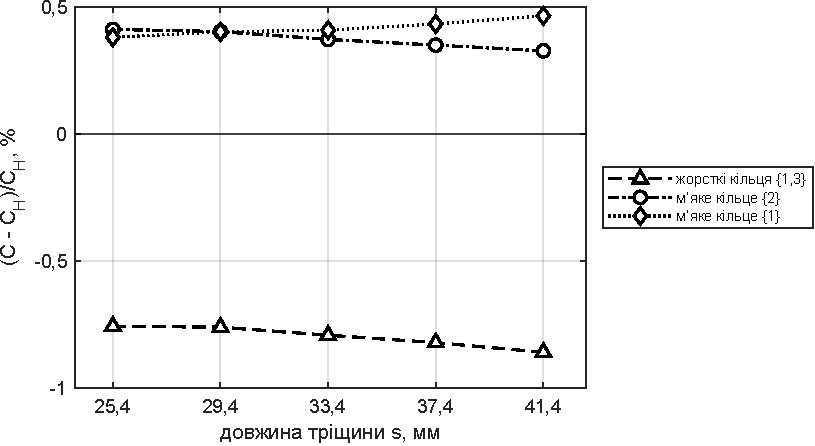
\includegraphics[width=\textwidth]{figures/M5_3_podatlyvist_UA.pdf}
 \caption{Відносна зміна податливості вздовж власних траєкторій S0--S4. Для енергетичного співвідношення потрібна похідна абсолютної різниці податливостей, а не лише відносного контрасту.}
 \label{fig:feedback-compliance}
\end{figure}

На останніх двох інтервалах розбіжність між оцінкою контрасту за різницями податливостей та середнім EDI-контрастом кінців інтервалу становить приблизно 0,03--0,5 відсоткового пункта; на початкових інтервалах розбіжність більша. Результат є додатковою діагностикою, а не новою межею похибки.

Загалом для фіксованої S4 геометрії прямий вплив матеріальної неоднорідності встановлює знак і основну величину енергетичного контрасту, а зміна геометрії частково його компенсує. Для локального кута спостерігається майже повна компенсація, проте накопичений напрямок та бічне зміщення не зникають. Перехресний план не розділяє внесок окремих змін ламаної, не встановлює чисельної похибки всіх членів та не визначає поведінку біля міжфазної межі. У наступному розділі розглянемо фактично прийняті власні траєкторії до дальших станів та їхні енергетичні й геометричні характеристики.

\chapter{Аналіз траєкторій поширення тріщин}
\label{ch:paths}
\reporttodo{Незалежні траєкторії, енергетичні та напрямні характеристики, межі продовження.}

\chapter{Узагальнення результатів і висновки}
\label{ch:conclusions}
\reporttodo{Підтверджені закономірності, обмеження та перспективи.}

\ifreportbibliography
  \printbibliography[heading=bibintoc,title={Список використаних джерел}]
\fi
% \appendix
% \chapter{Додаткові матеріали чисельної верифікації}
\reporttodo{Матеріали буде відібрано після інвентаризації.}

\end{document}
